\chapter[\leavevmode\newline Results]{Results}
\chaptermark{Results}
\label{chap:Chapter_6}

\section{Invariant mass distribution of $B^0_S$}
\subsection{$p_T$ bins}

\begin{figure}
	\centering
	\begin{subfigure}[t]{0.8\textwidth}
		\raisebox{-\height}{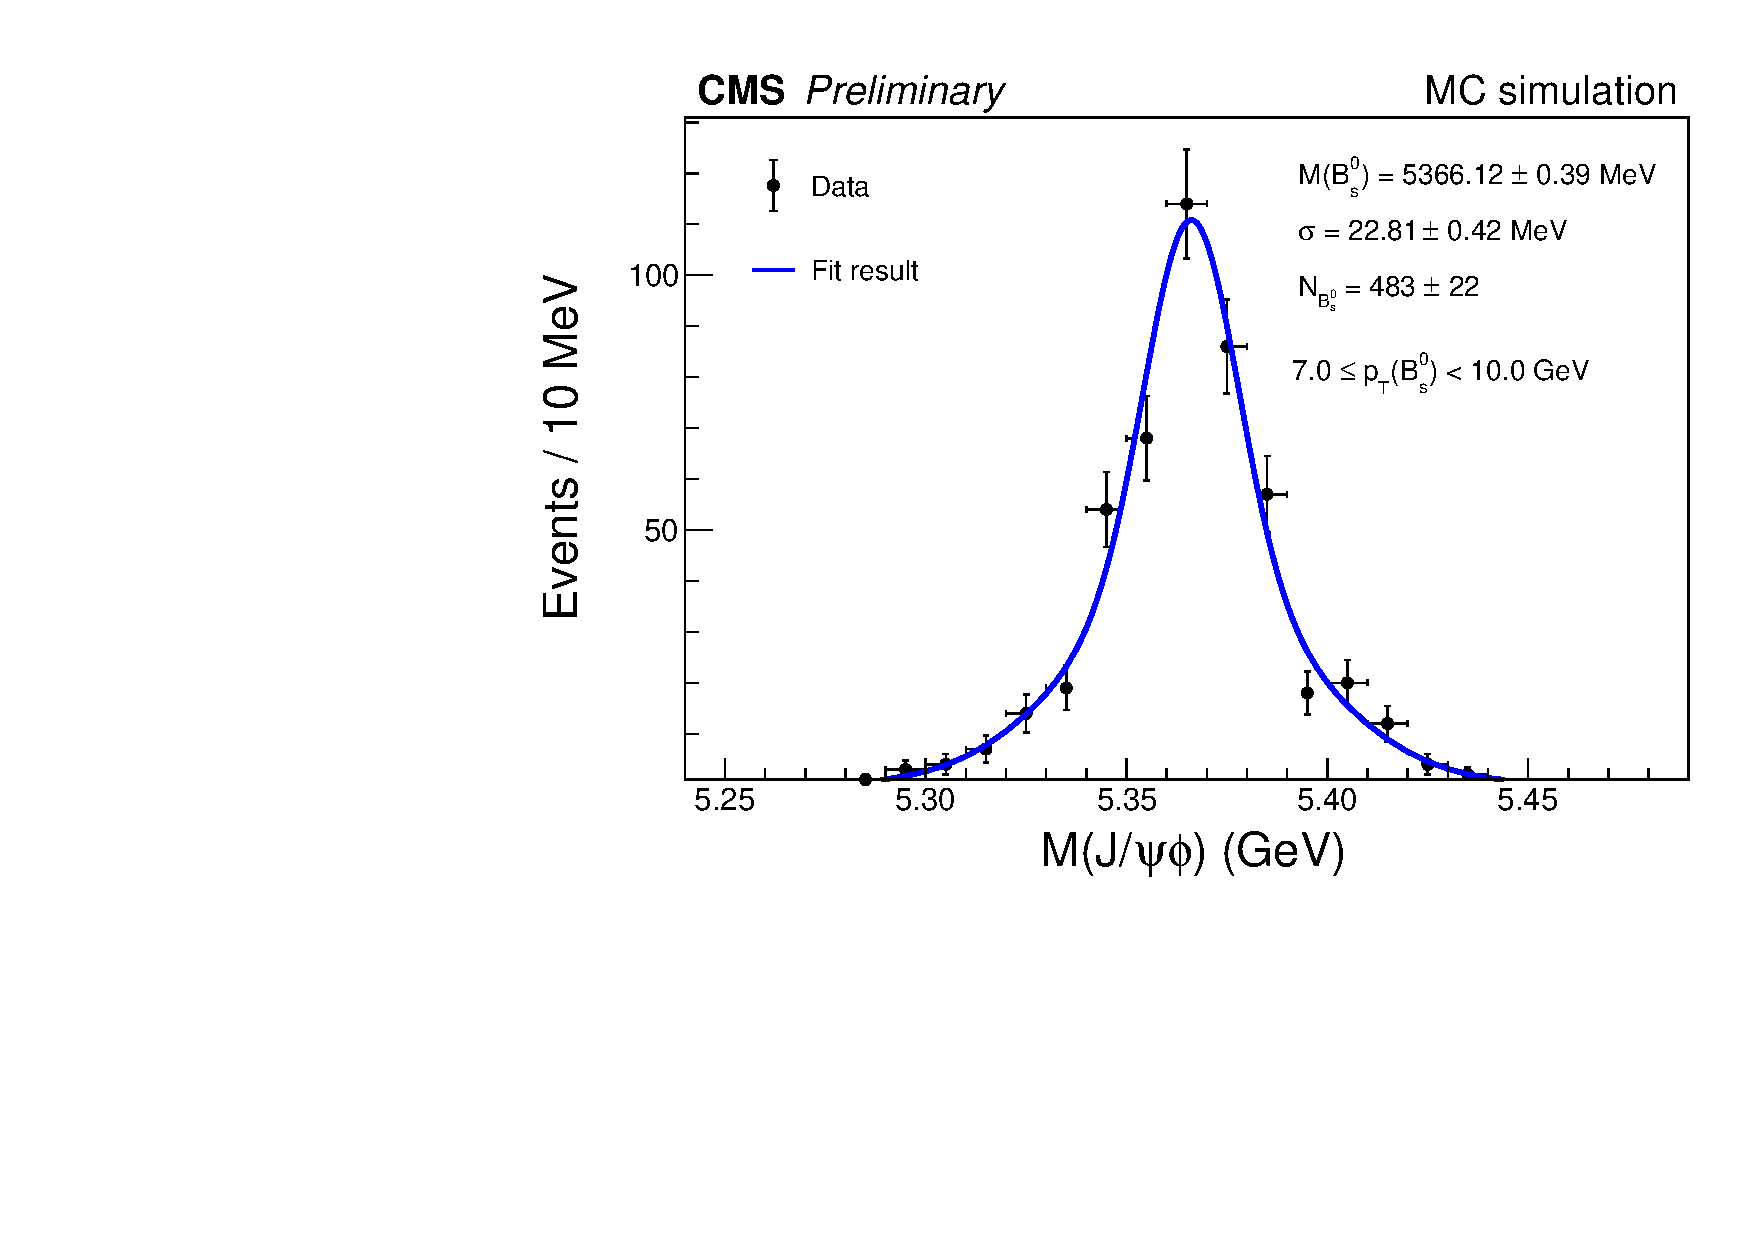
\includegraphics[width=0.49\textwidth]{MainContent/Figs/mass/mass_BsFitMC_best1_ptbins_7_10.PDF}}
		\raisebox{-\height}{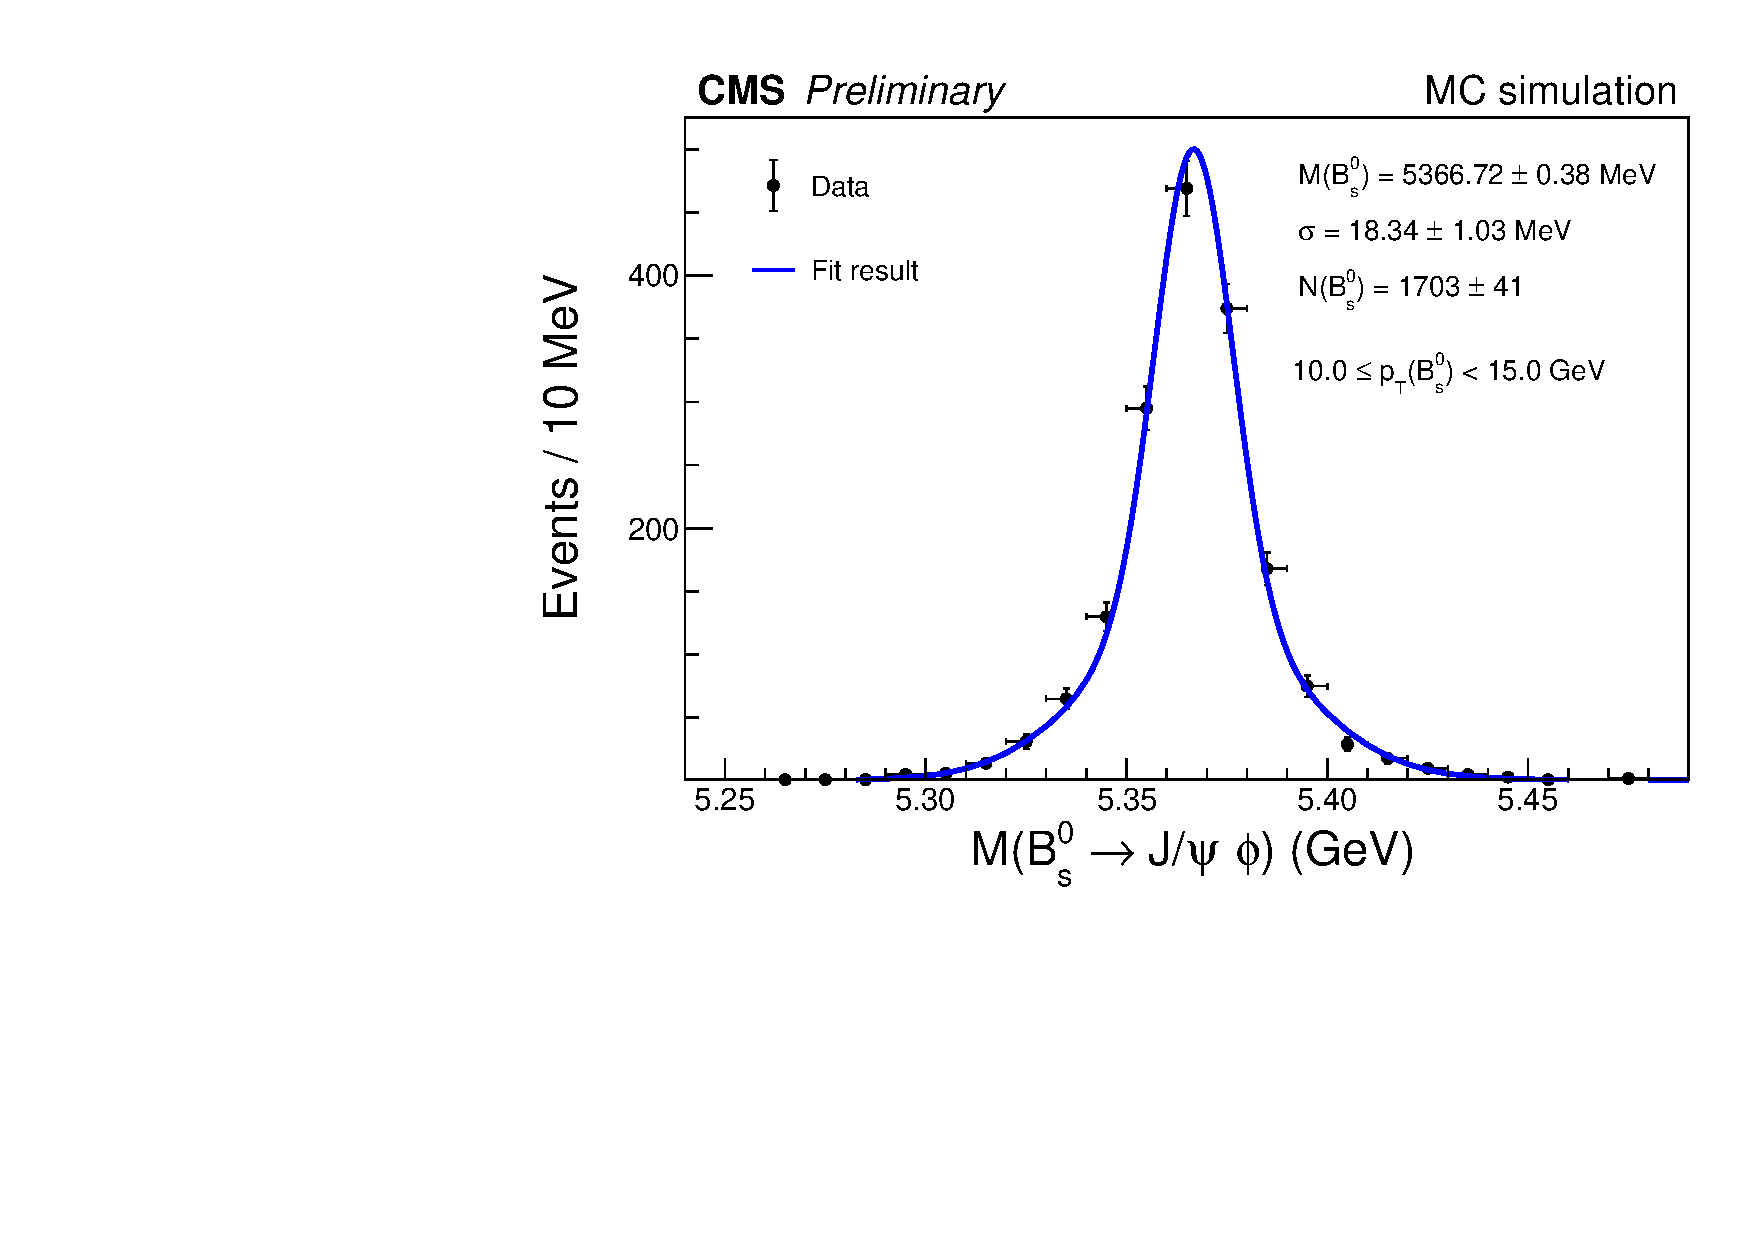
\includegraphics[width=0.49\textwidth]{MainContent/Figs/mass/mass_BsFitMC_best1_ptbins_10_15.PDF}}%
		\vspace{.6ex}
			\raisebox{-\height}{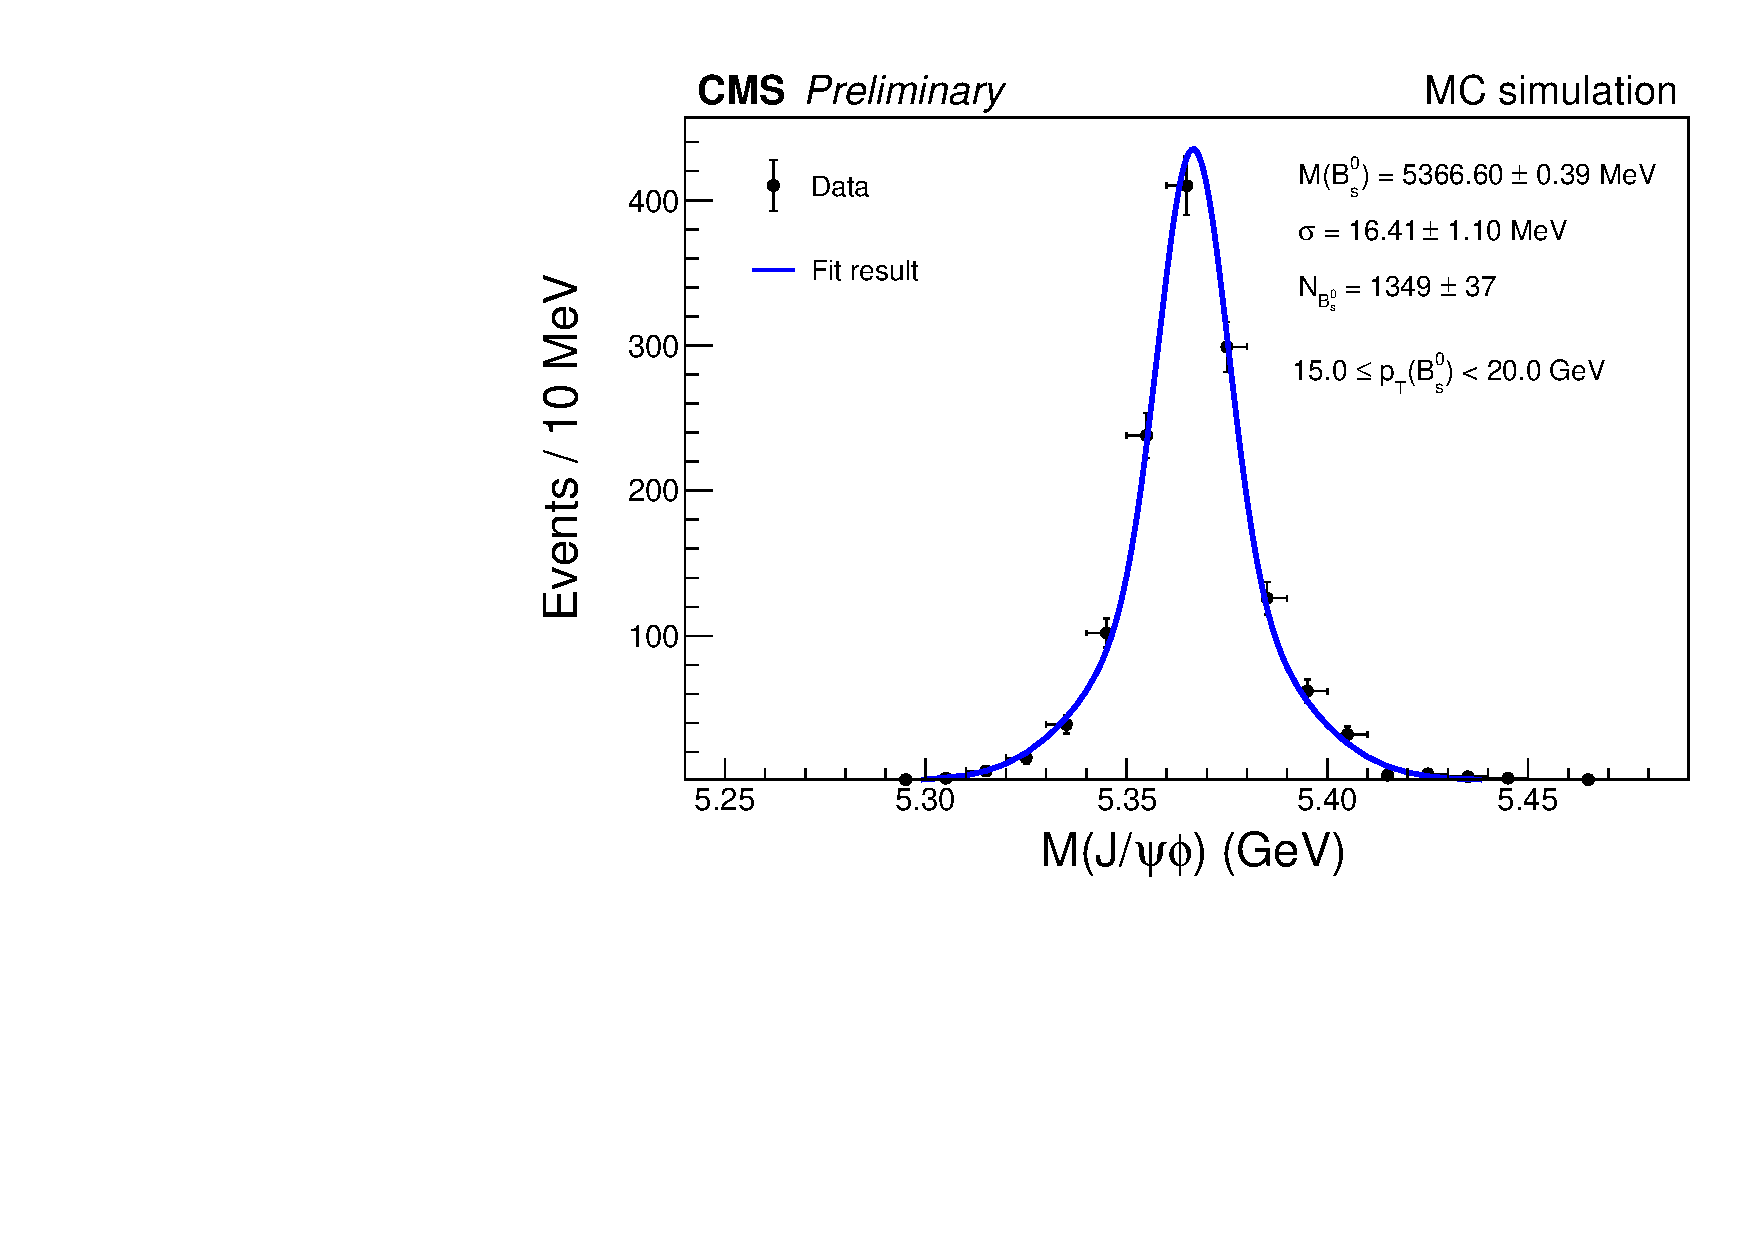
\includegraphics[width=0.49\textwidth]{MainContent/Figs/mass/mass_BsFitMC_best1_ptbins_15_20.PDF}}
		\raisebox{-\height}{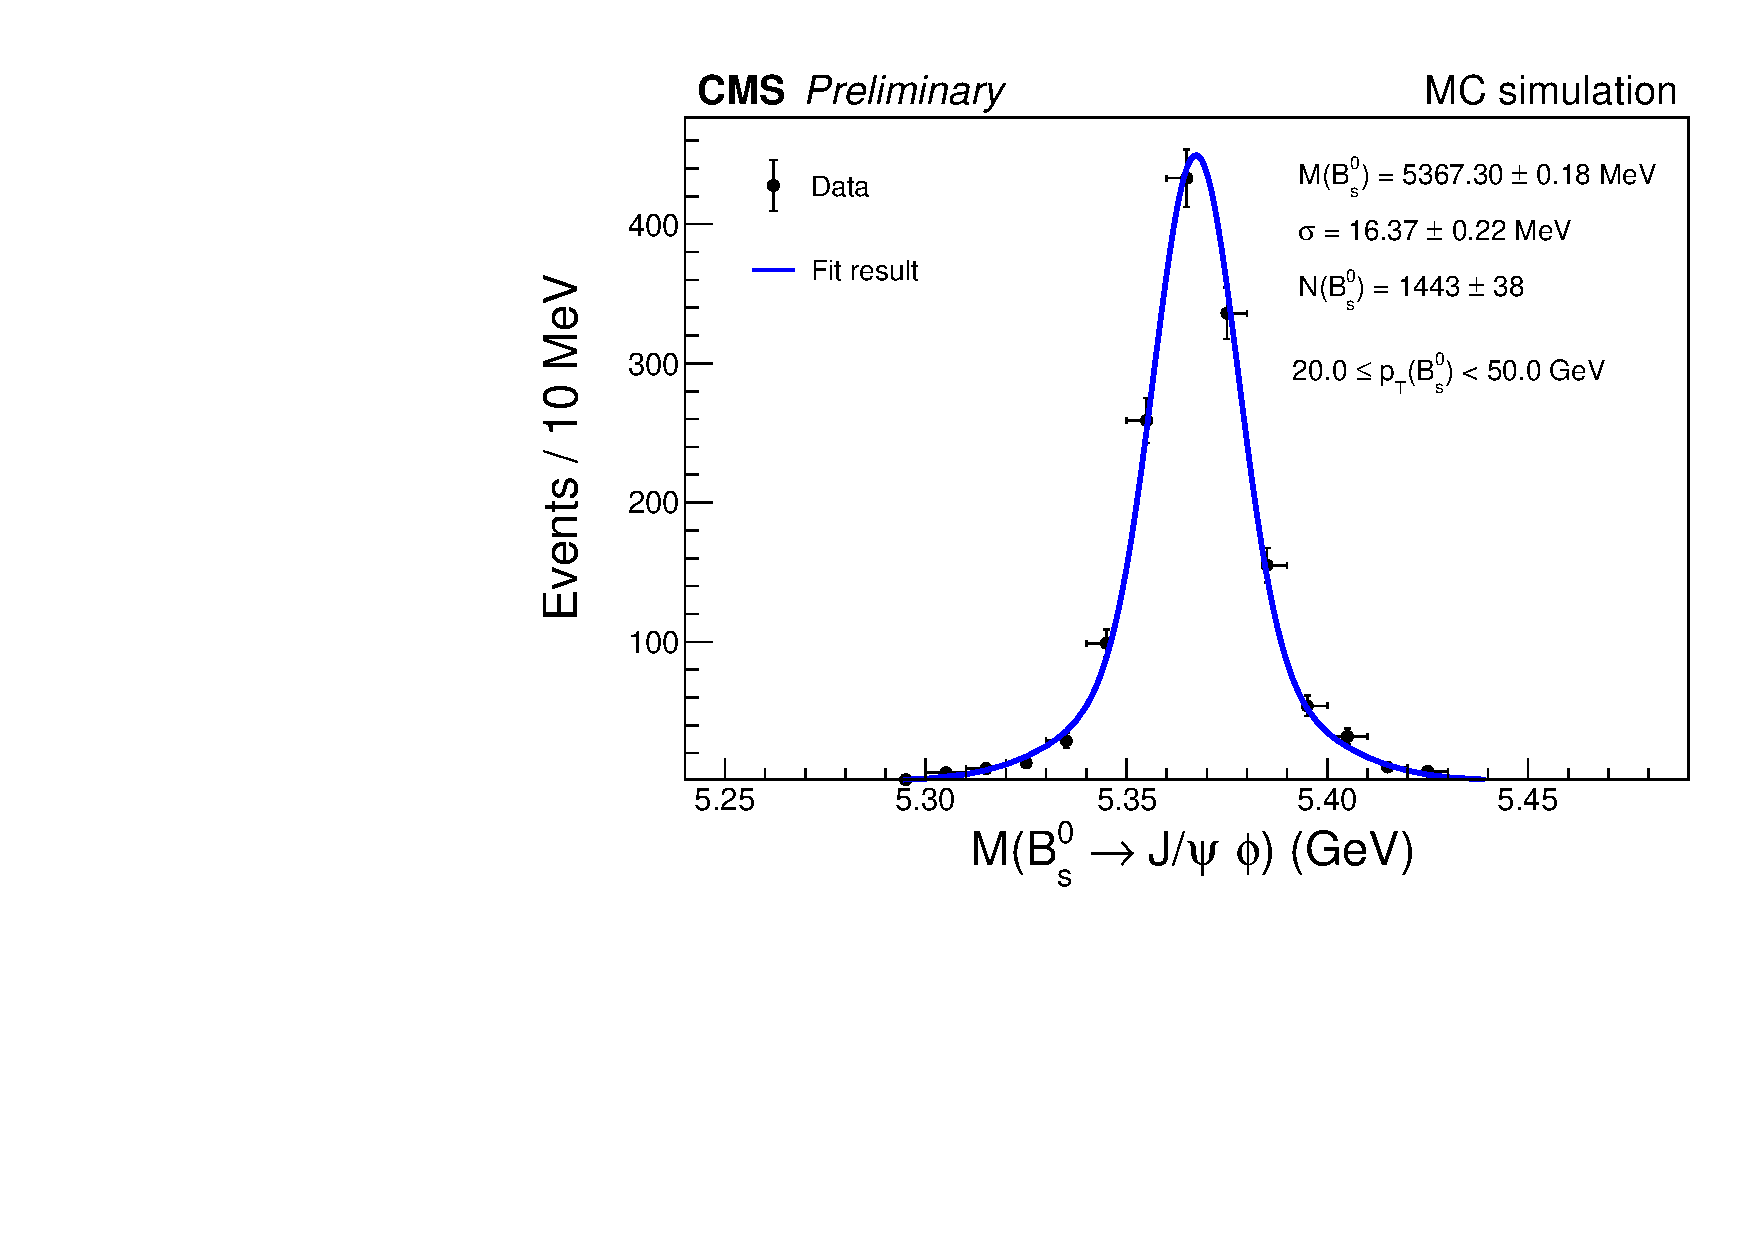
\includegraphics[width=0.49\textwidth]{MainContent/Figs/mass/mass_BsFitMC_best1_ptbins_20_50.PDF}}%
	\end{subfigure}
	\hfill
	\begin{subfigure}[t]{0.8\textwidth}
		\raisebox{-\height}{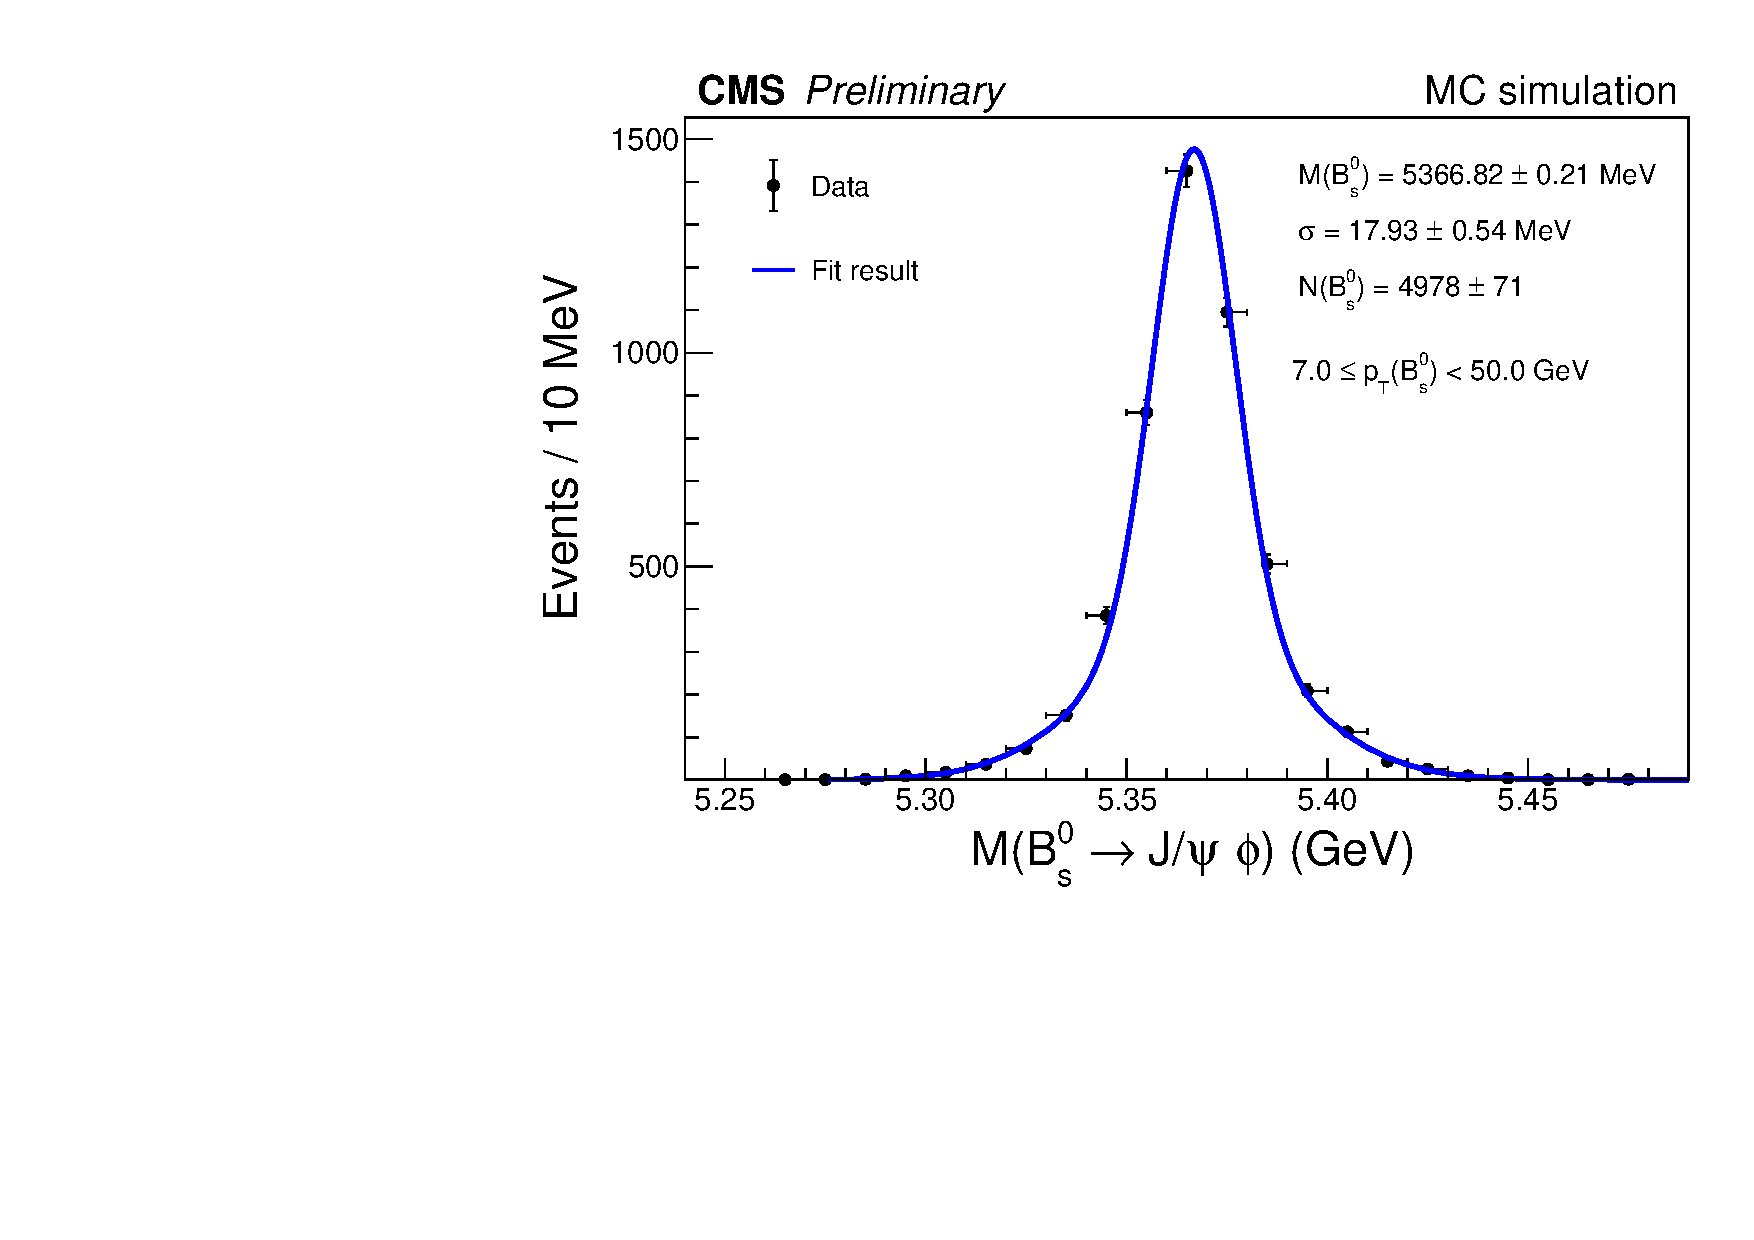
\includegraphics[width=\textwidth]{MainContent/Figs/mass/mass_BsFitMC_best1_ptbins_7_50.PDF}}
		
	\end{subfigure}
	\caption{Invariant mass spectra for the $B^0_s$ meson using the data from the MC simulation and considering the different bins for $p_T$. }
	%%%%%%%%%%%%%%%%%%%%%%%%%%%%%%%%%%%%second row
	
\end{figure}


\begin{figure}
	\centering
	\begin{subfigure}[t]{0.8\textwidth}
		\raisebox{-\height}{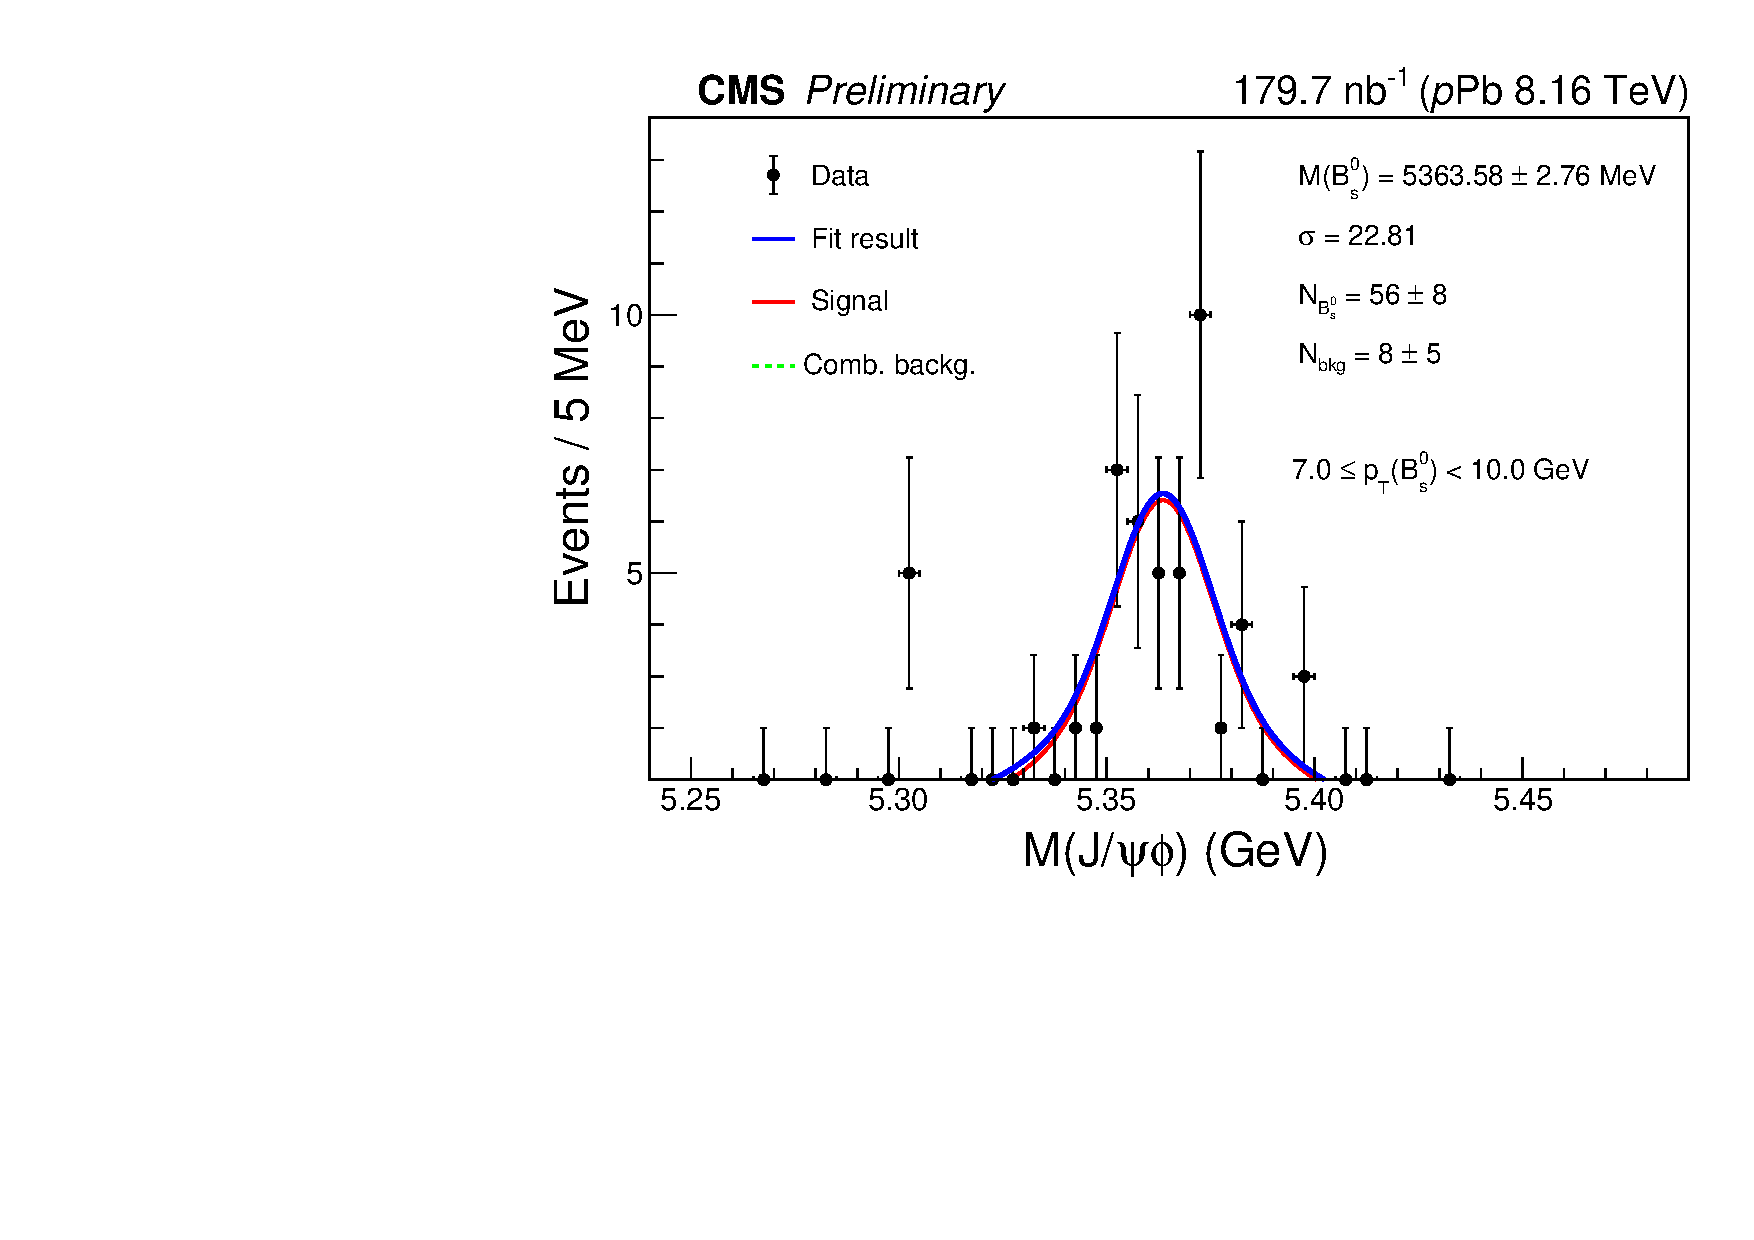
\includegraphics[width=0.49\textwidth]{MainContent/Figs/mass/mass_BsFit_ptbins_7_10.PDF}}
		\raisebox{-\height}{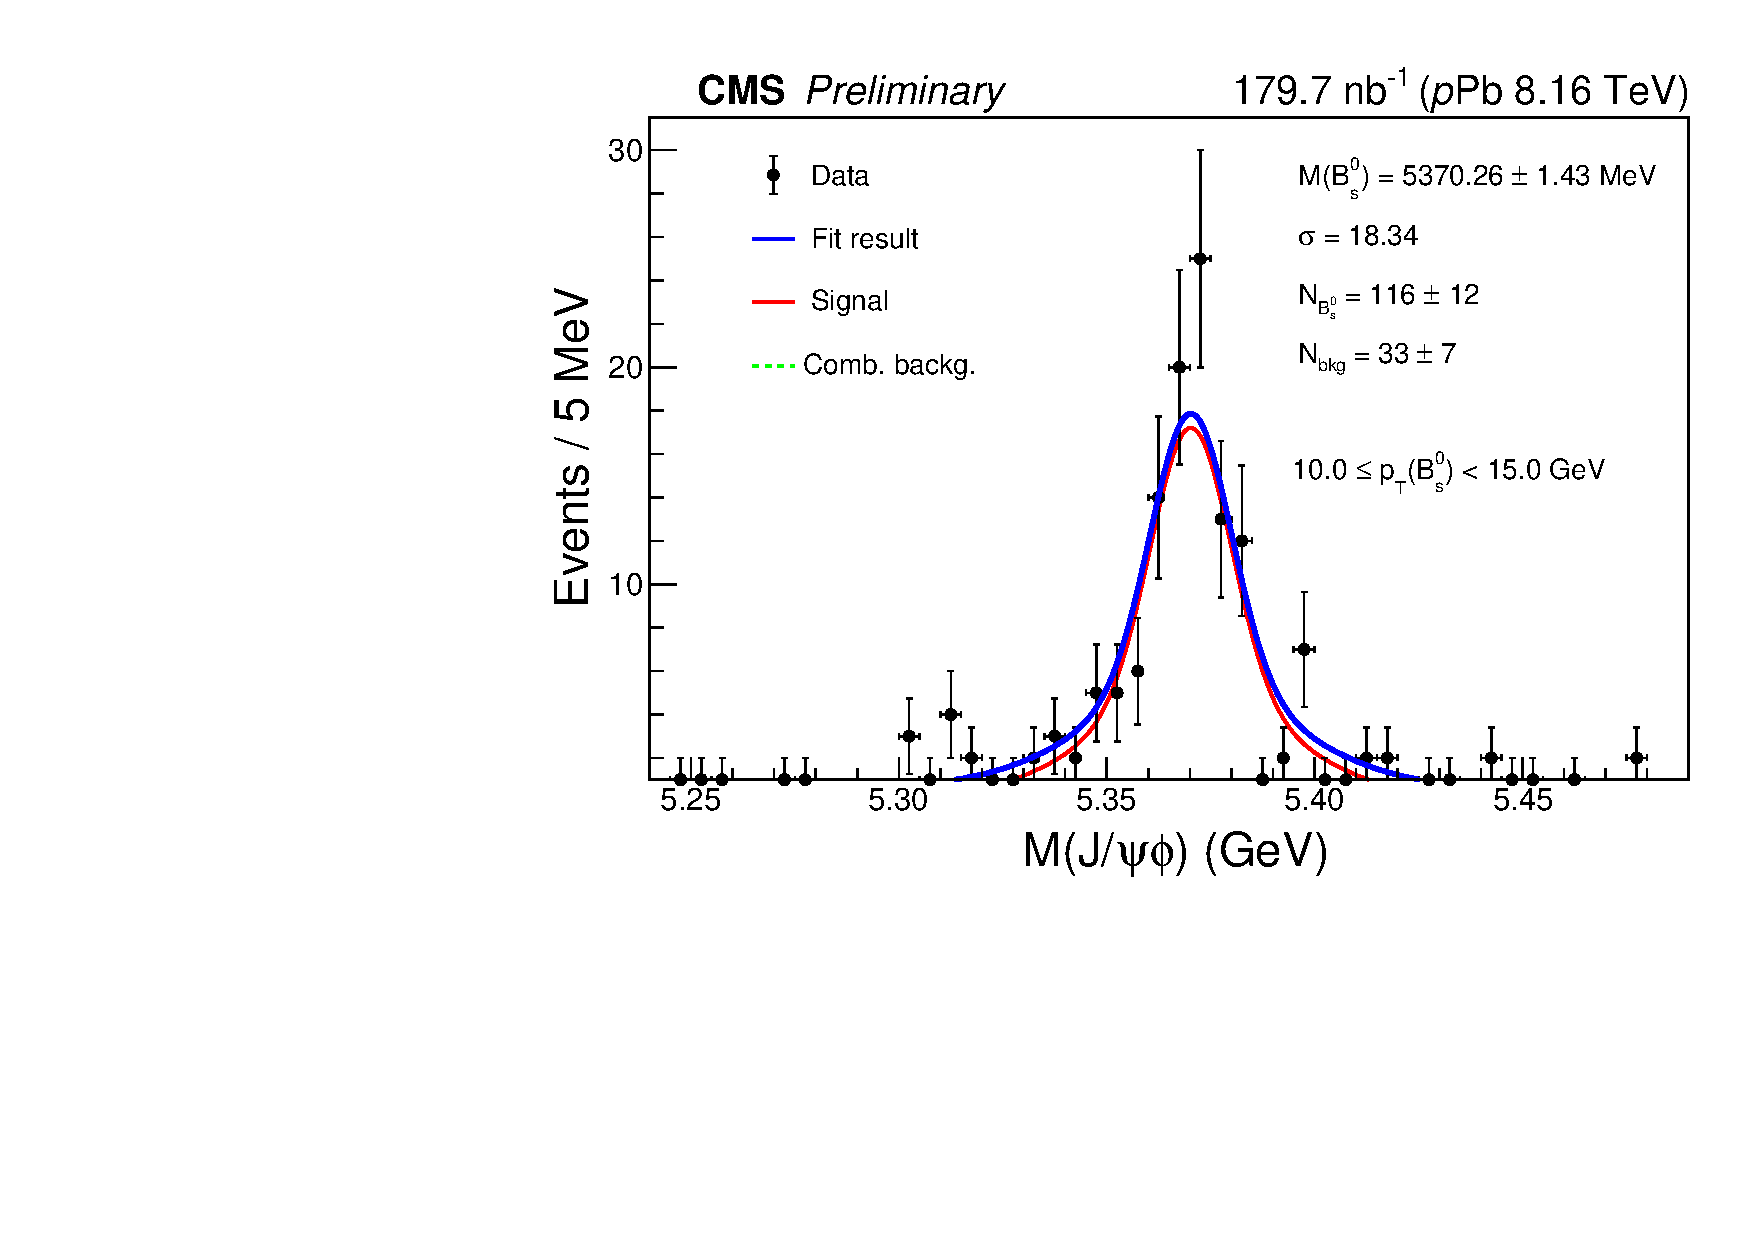
\includegraphics[width=0.49\textwidth]{MainContent/Figs/mass/mass_BsFit_ptbins_10_15.PDF}}%
		\vspace{.6ex}
		\raisebox{-\height}{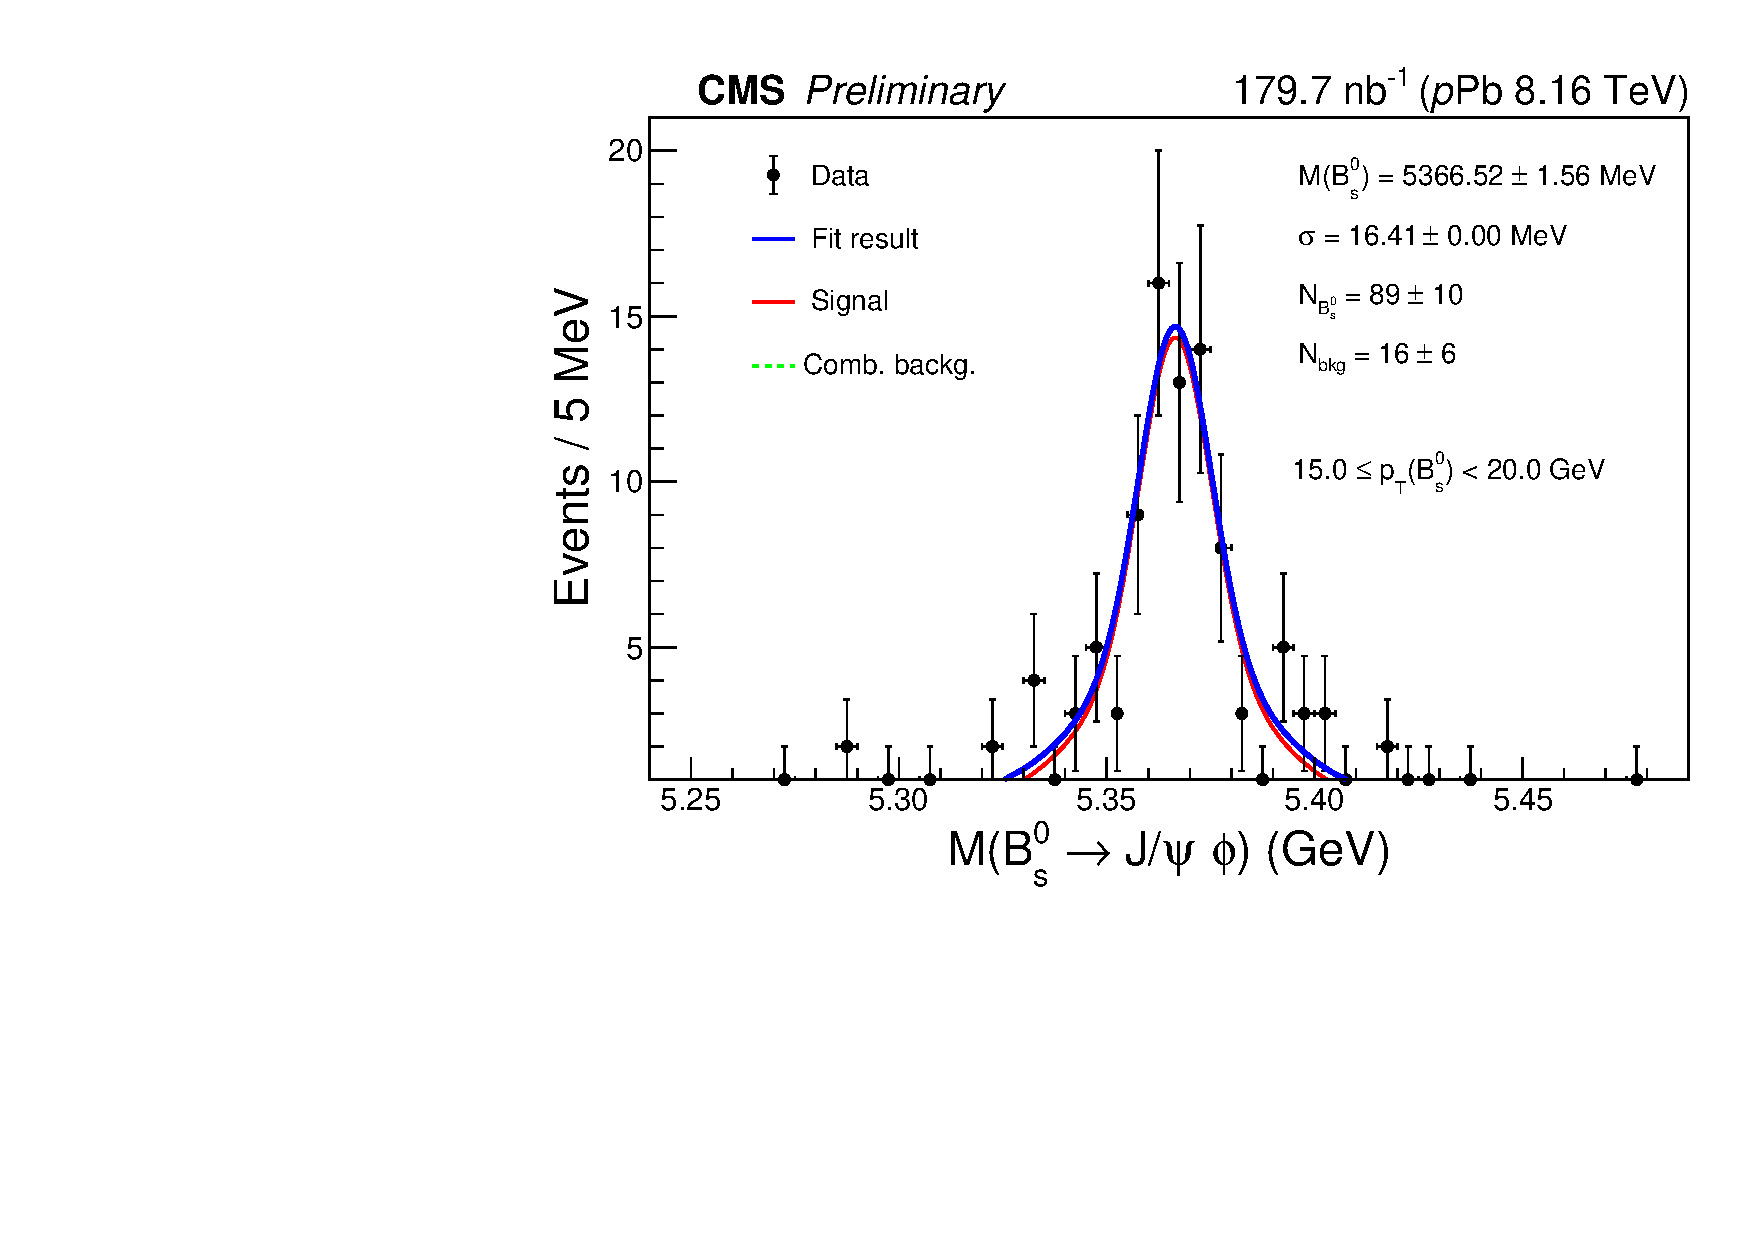
\includegraphics[width=0.49\textwidth]{MainContent/Figs/mass/mass_BsFit_ptbins_15_20.PDF}}
		\raisebox{-\height}{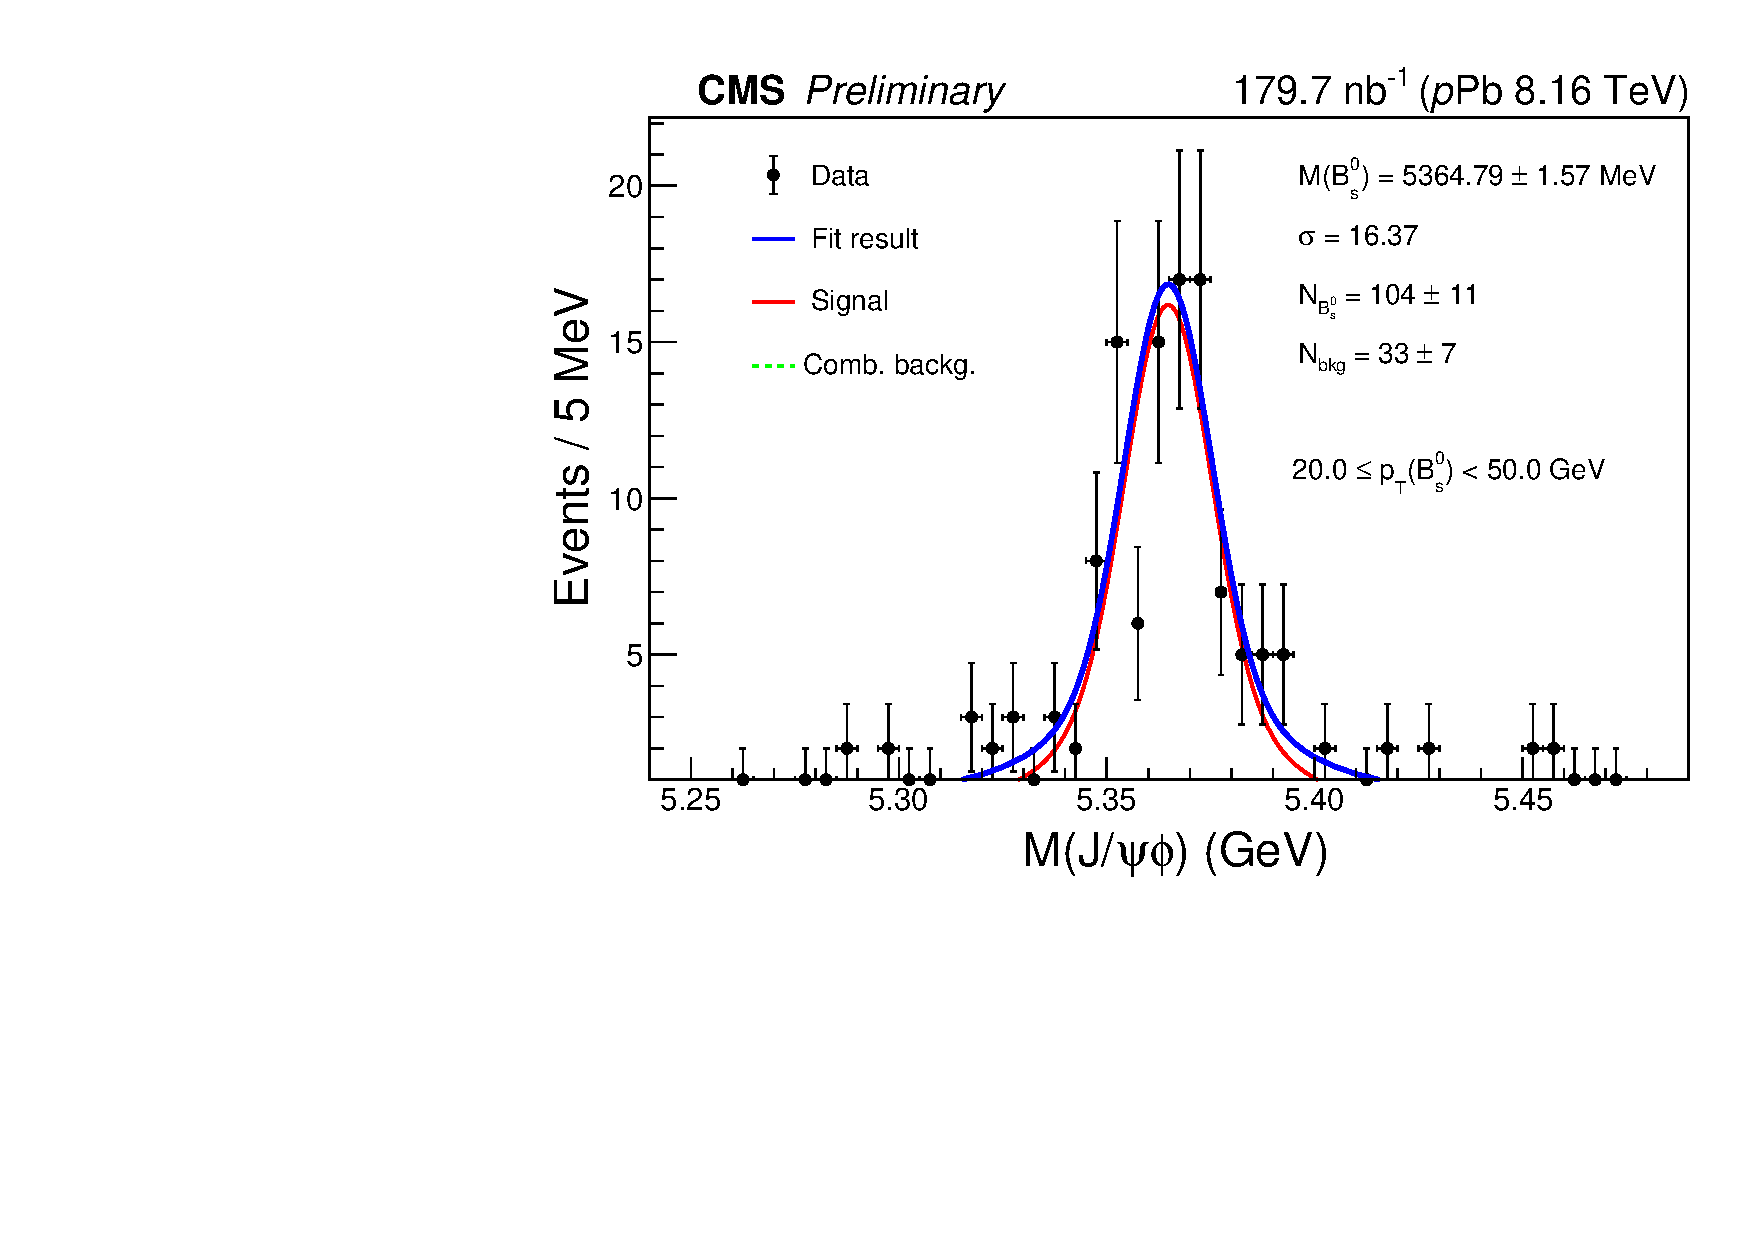
\includegraphics[width=0.49\textwidth]{MainContent/Figs/mass/mass_BsFit_ptbins_20_50.PDF}}%
	\end{subfigure}
	\hfill
	\begin{subfigure}[t]{0.8\textwidth}
		\raisebox{-\height}{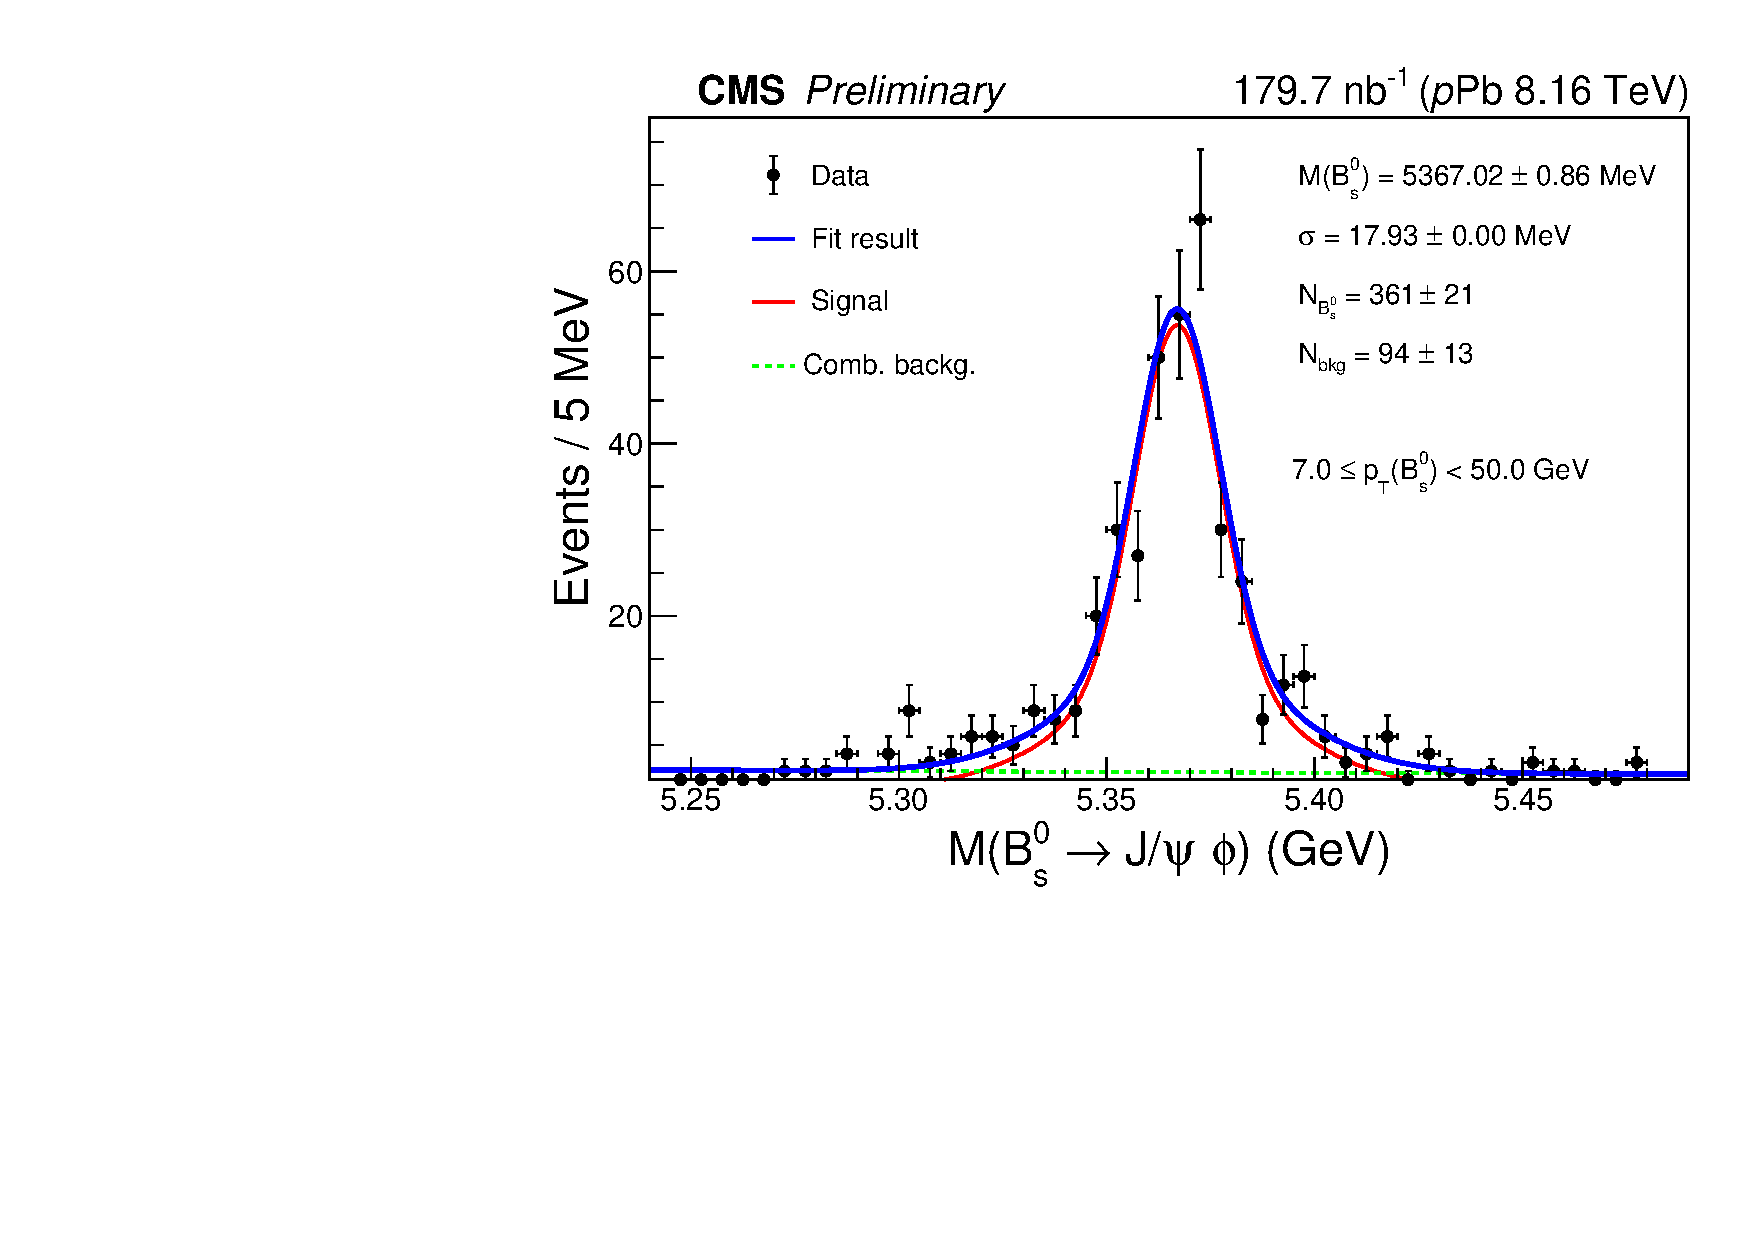
\includegraphics[width=\textwidth]{MainContent/Figs/mass/mass_BsFit_ptbins_7_50.PDF}}
		
	\end{subfigure}
	\caption{Invariant mass spectra for the $B^0_s$ meson using the data from p-Pb collision and considering the different bins for $p_T$. }
	%%%%%%%%%%%%%%%%%%%%%%%%%%%%%%%%%%%%second row
	
\end{figure}

\begin{figure}
	\centering
	\begin{subfigure}[t]{0.8\textwidth}
		\raisebox{-\height}{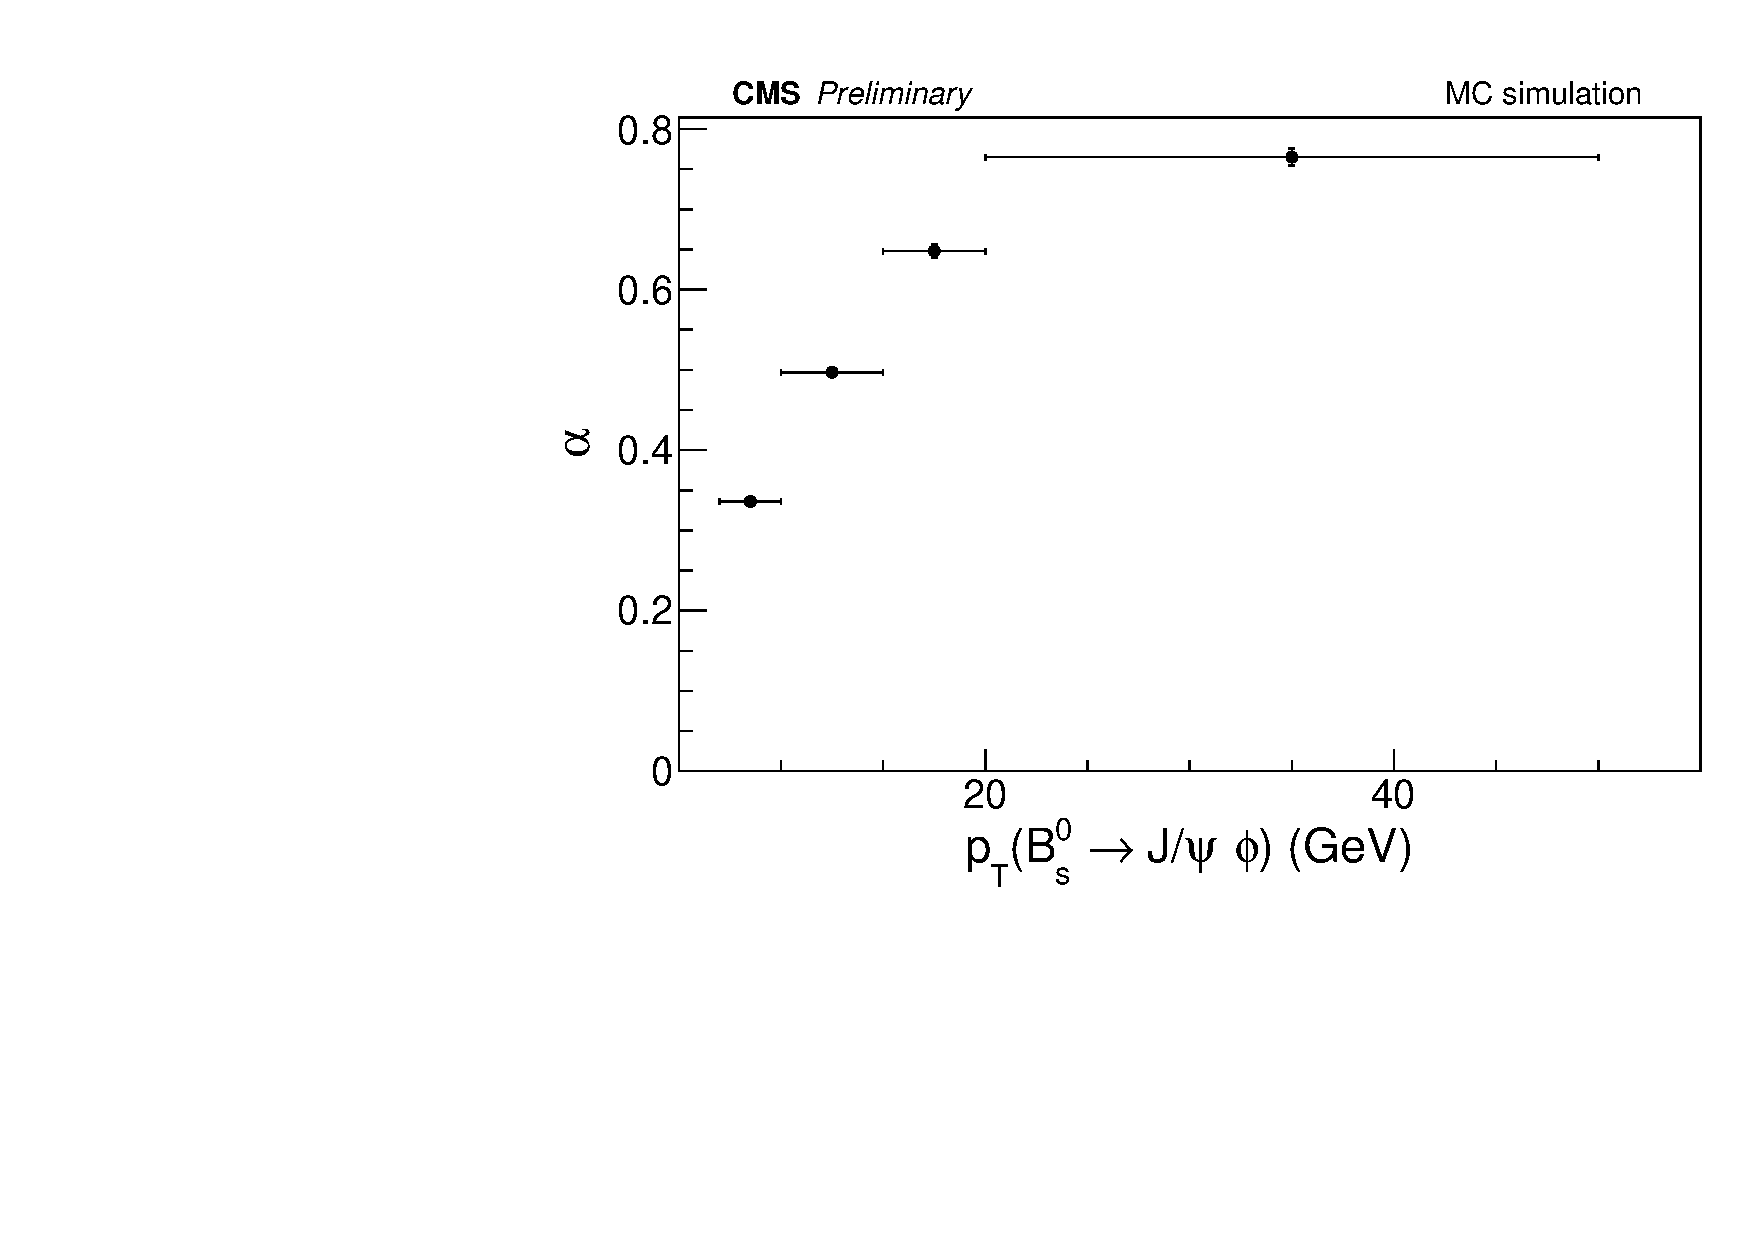
\includegraphics[width=0.49\textwidth]{MainContent/Figs/effy/Bseffy_prefilter.PDF}}
		\raisebox{-\height}{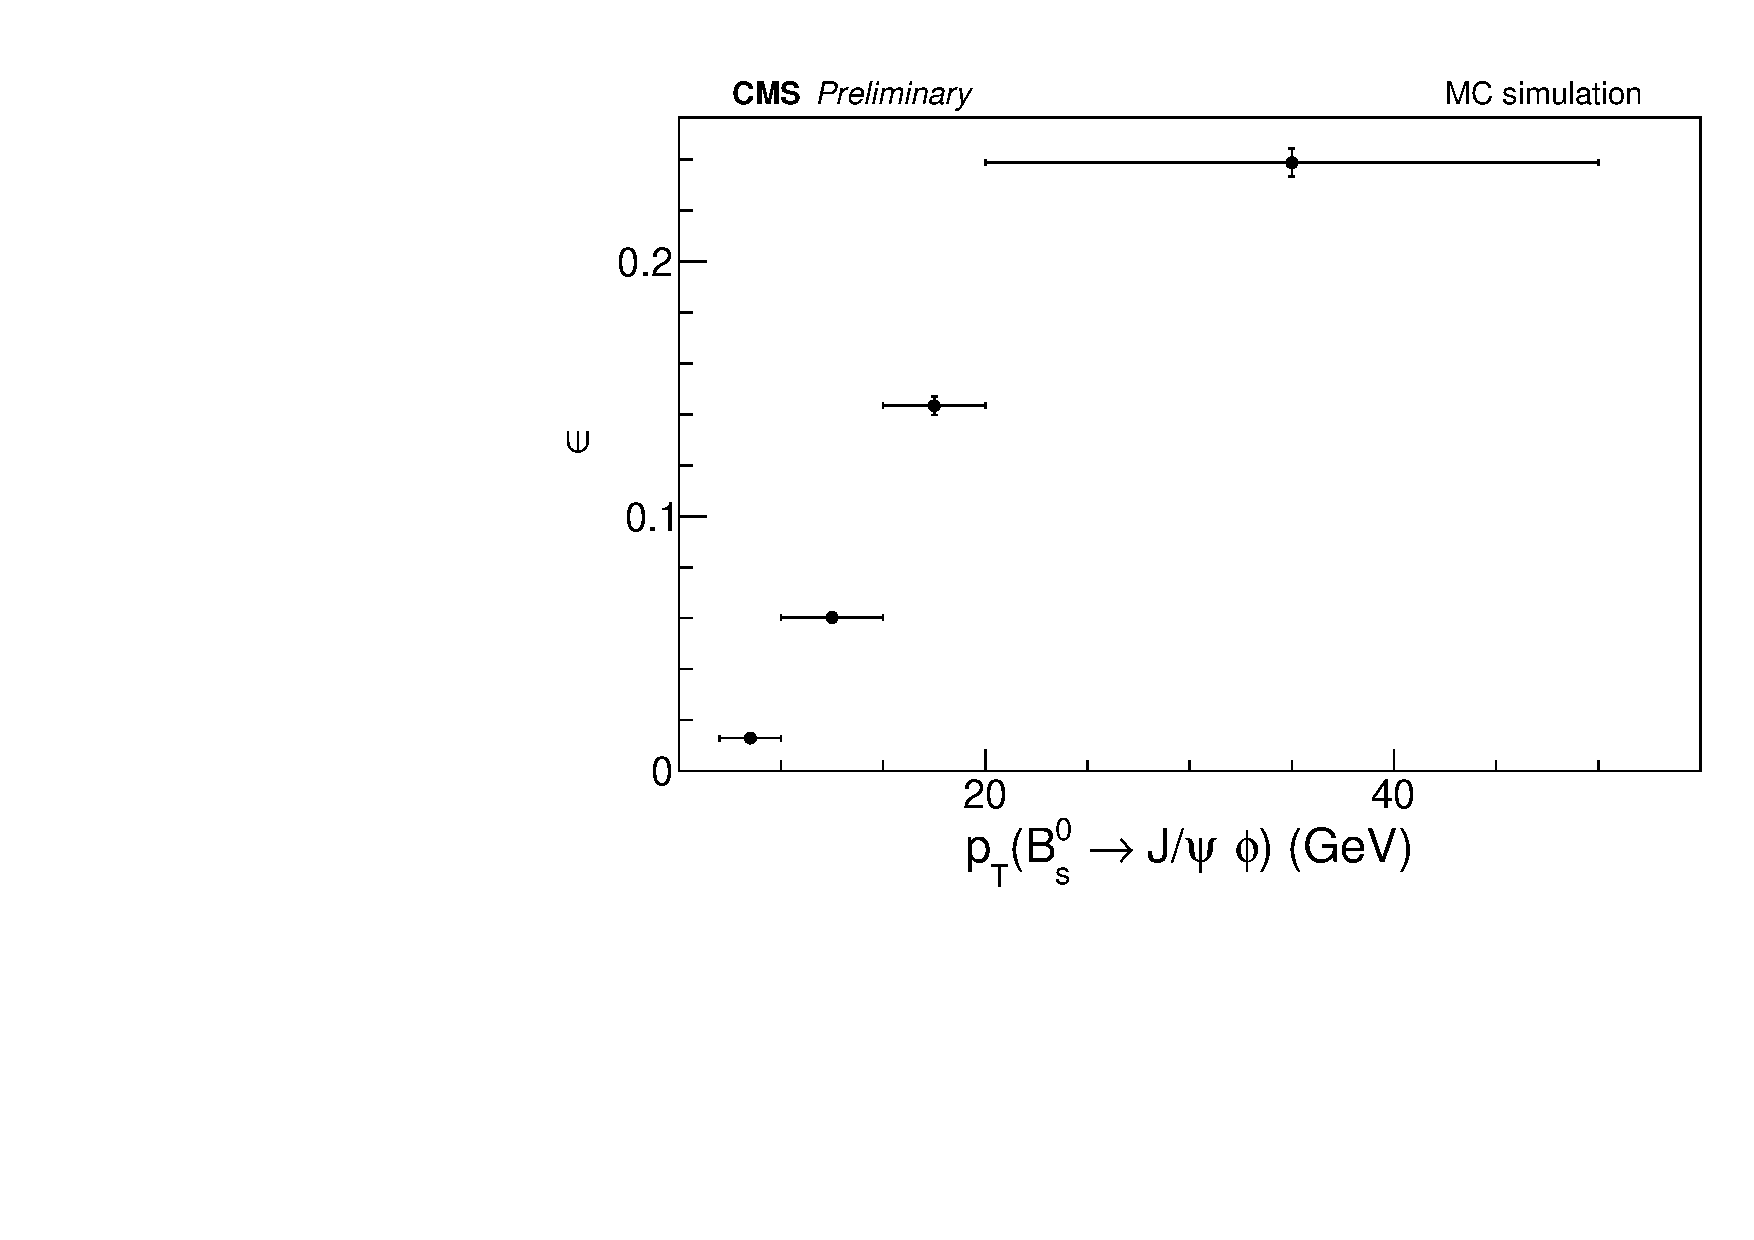
\includegraphics[width=0.49\textwidth]{MainContent/Figs/effy/Bseffy_reco.PDF}}%
	\end{subfigure}
	\hfill
	\begin{subfigure}[t]{0.8\textwidth}
		\raisebox{-\height}{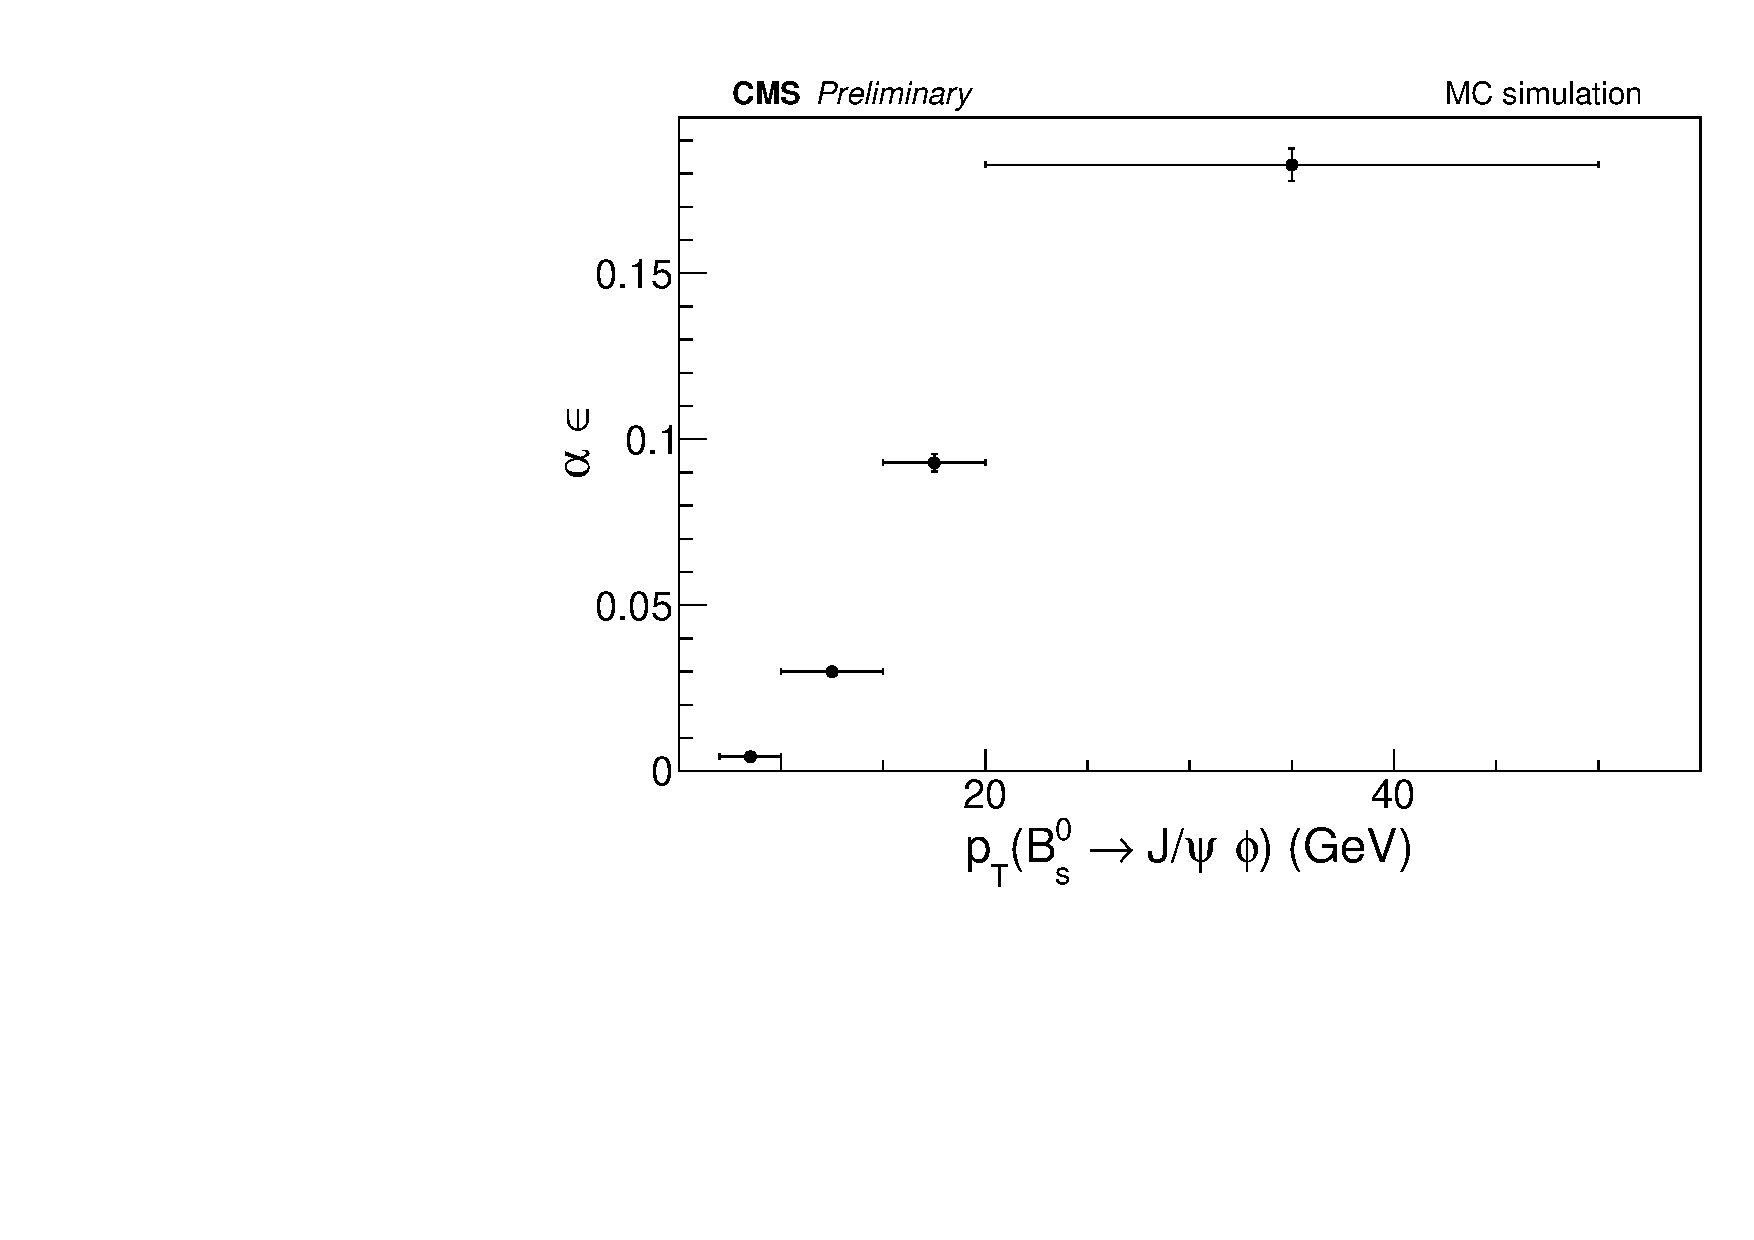
\includegraphics[width=\textwidth]{MainContent/Figs/effy/Bseffy_Total.PDF}}
		
	\end{subfigure}
	\caption{Acceptance, efficiency and total efficiency for the MC simulation.}
	%%%%%%%%%%%%%%%%%%%%%%%%%%%%%%%%%%%%second row
	
\end{figure}

\begin{figure}
	\centering
	\begin{subfigure}[t]{0.8\textwidth}
		\raisebox{-\height}{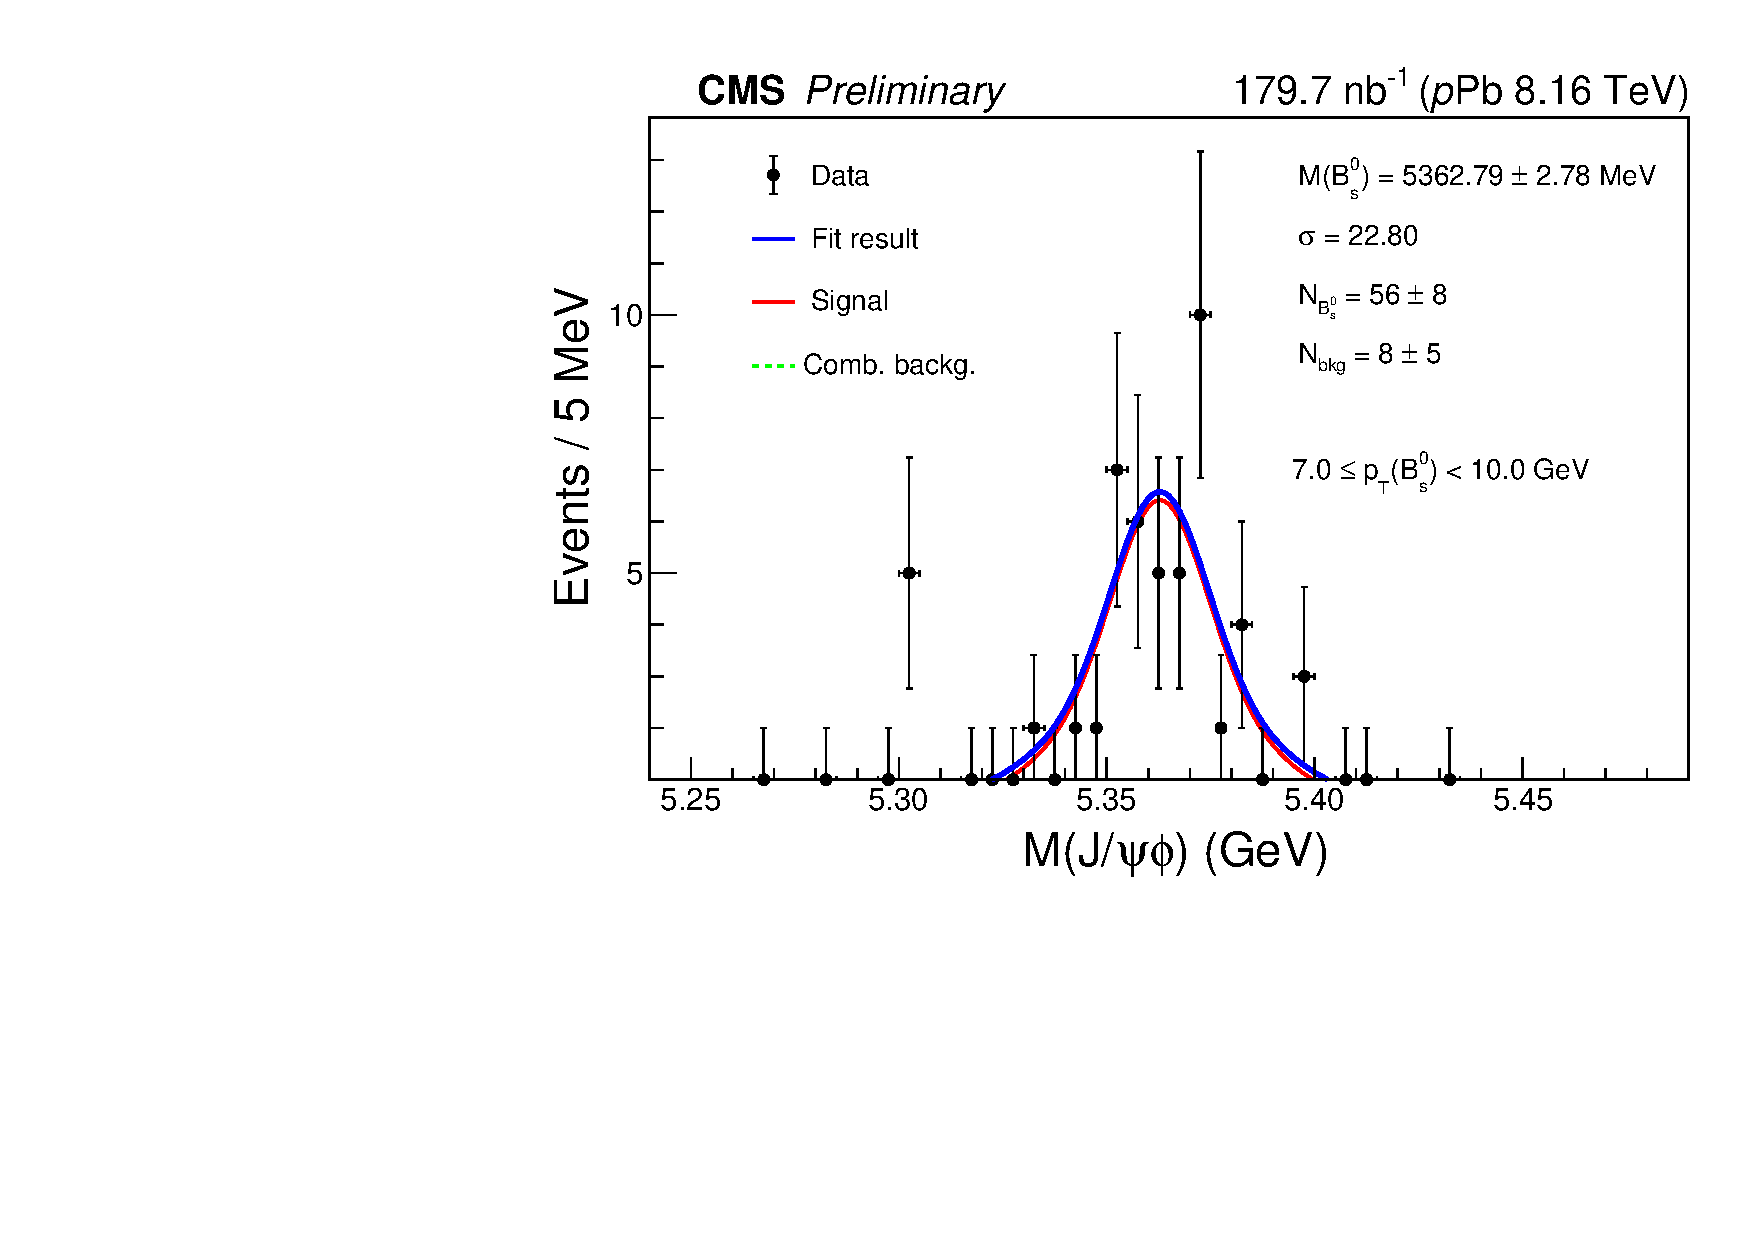
\includegraphics[width=0.49\textwidth]{MainContent/Figs/mass/mass_BsFit_ptbins_sysbkg_7_10.PDF}}
		\raisebox{-\height}{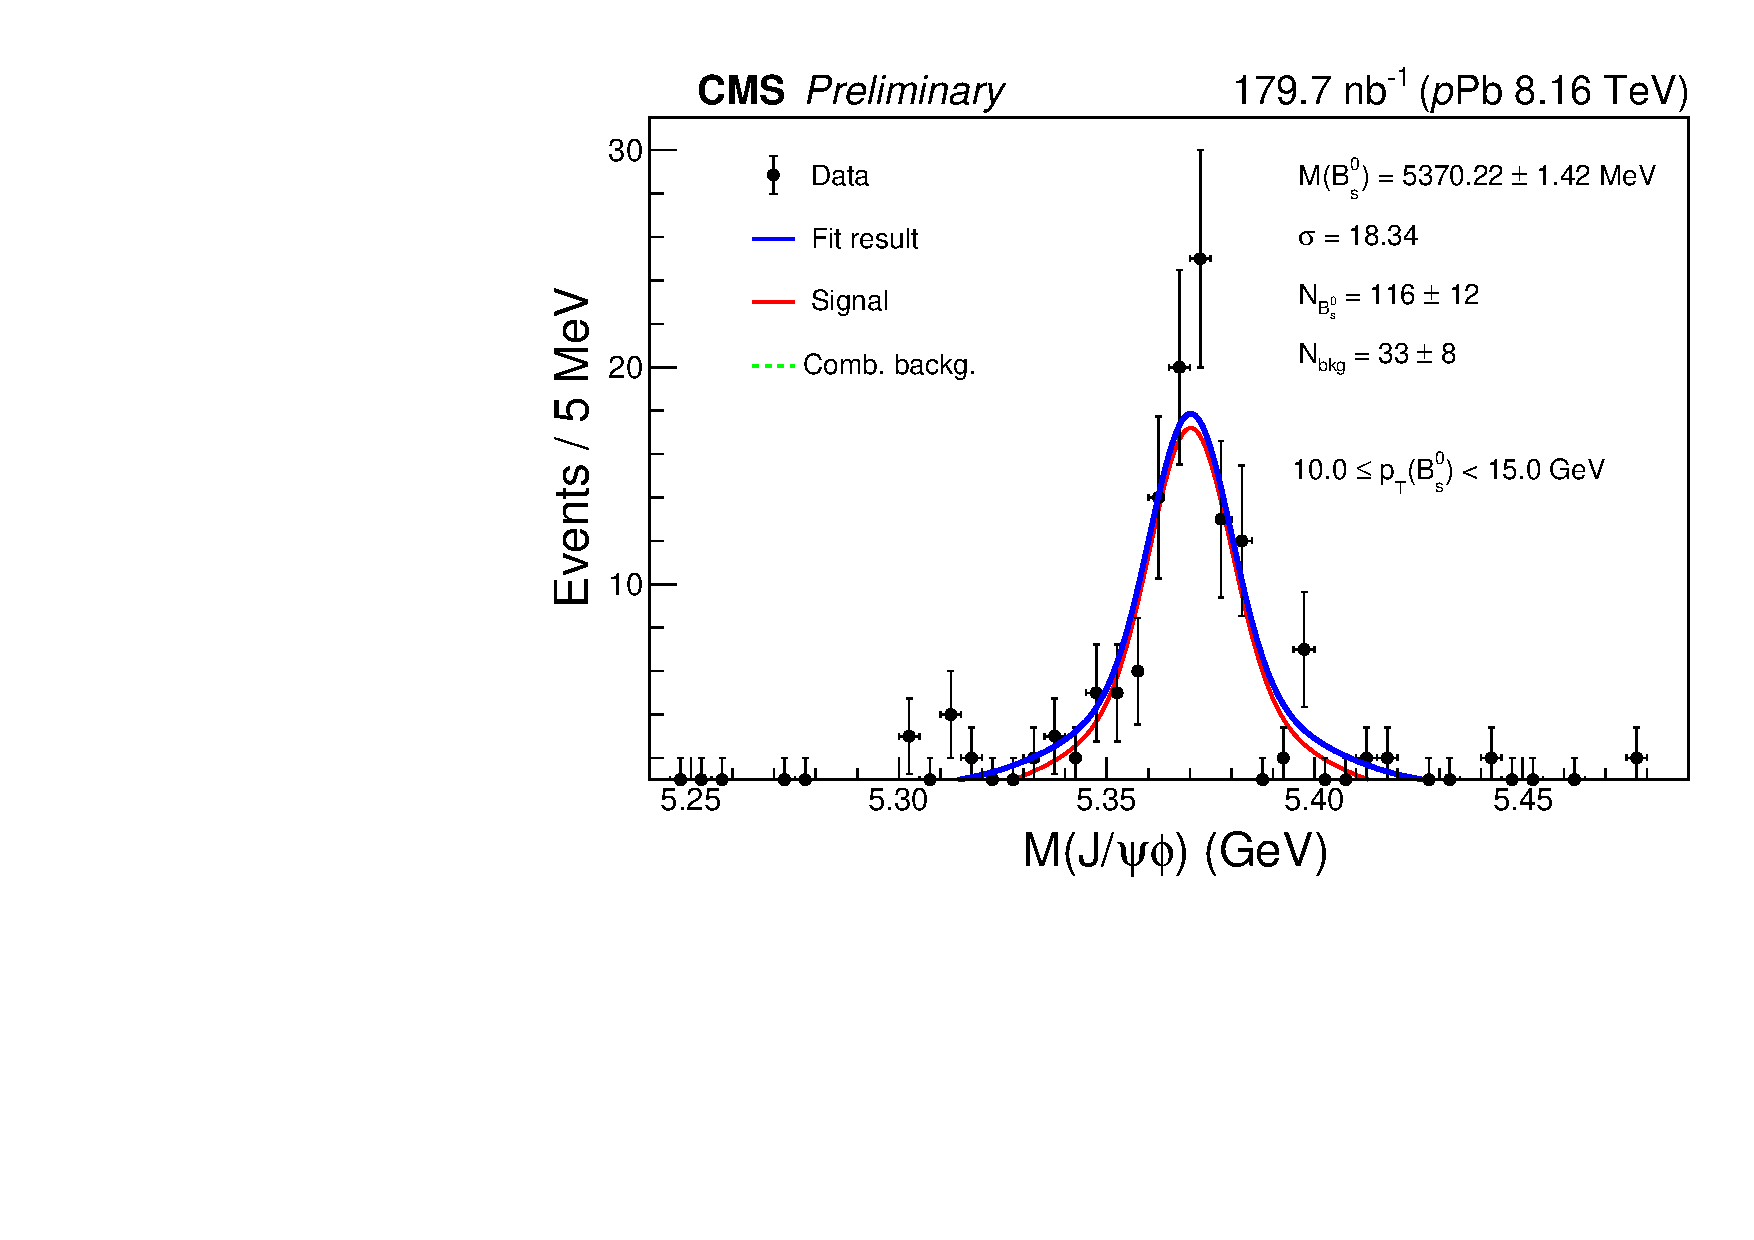
\includegraphics[width=0.49\textwidth]{MainContent/Figs/mass/mass_BsFit_ptbins_sysbkg_10_15.PDF}}%
		\vspace{.6ex}
		\raisebox{-\height}{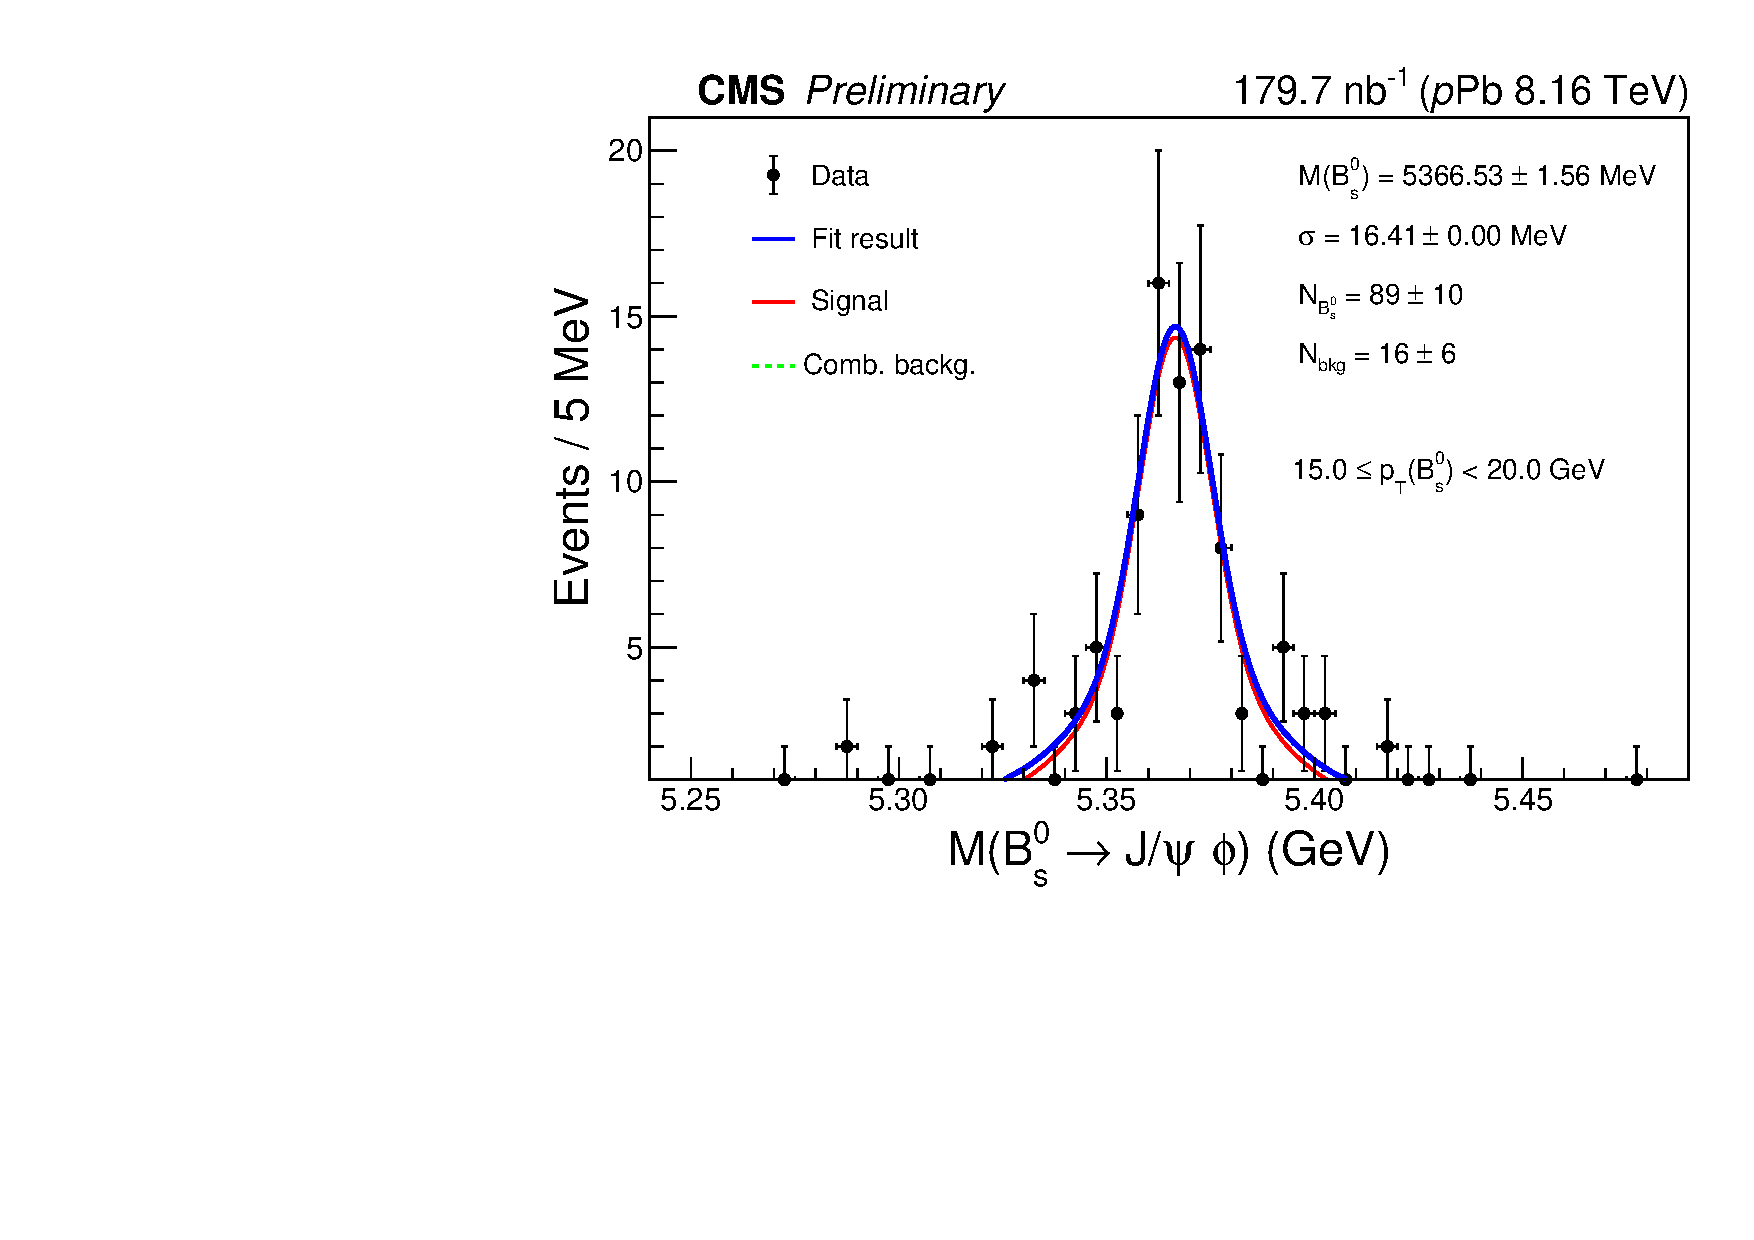
\includegraphics[width=0.49\textwidth]{MainContent/Figs/mass/mass_BsFit_ptbins_sysbkg_15_20.PDF}}
		\raisebox{-\height}{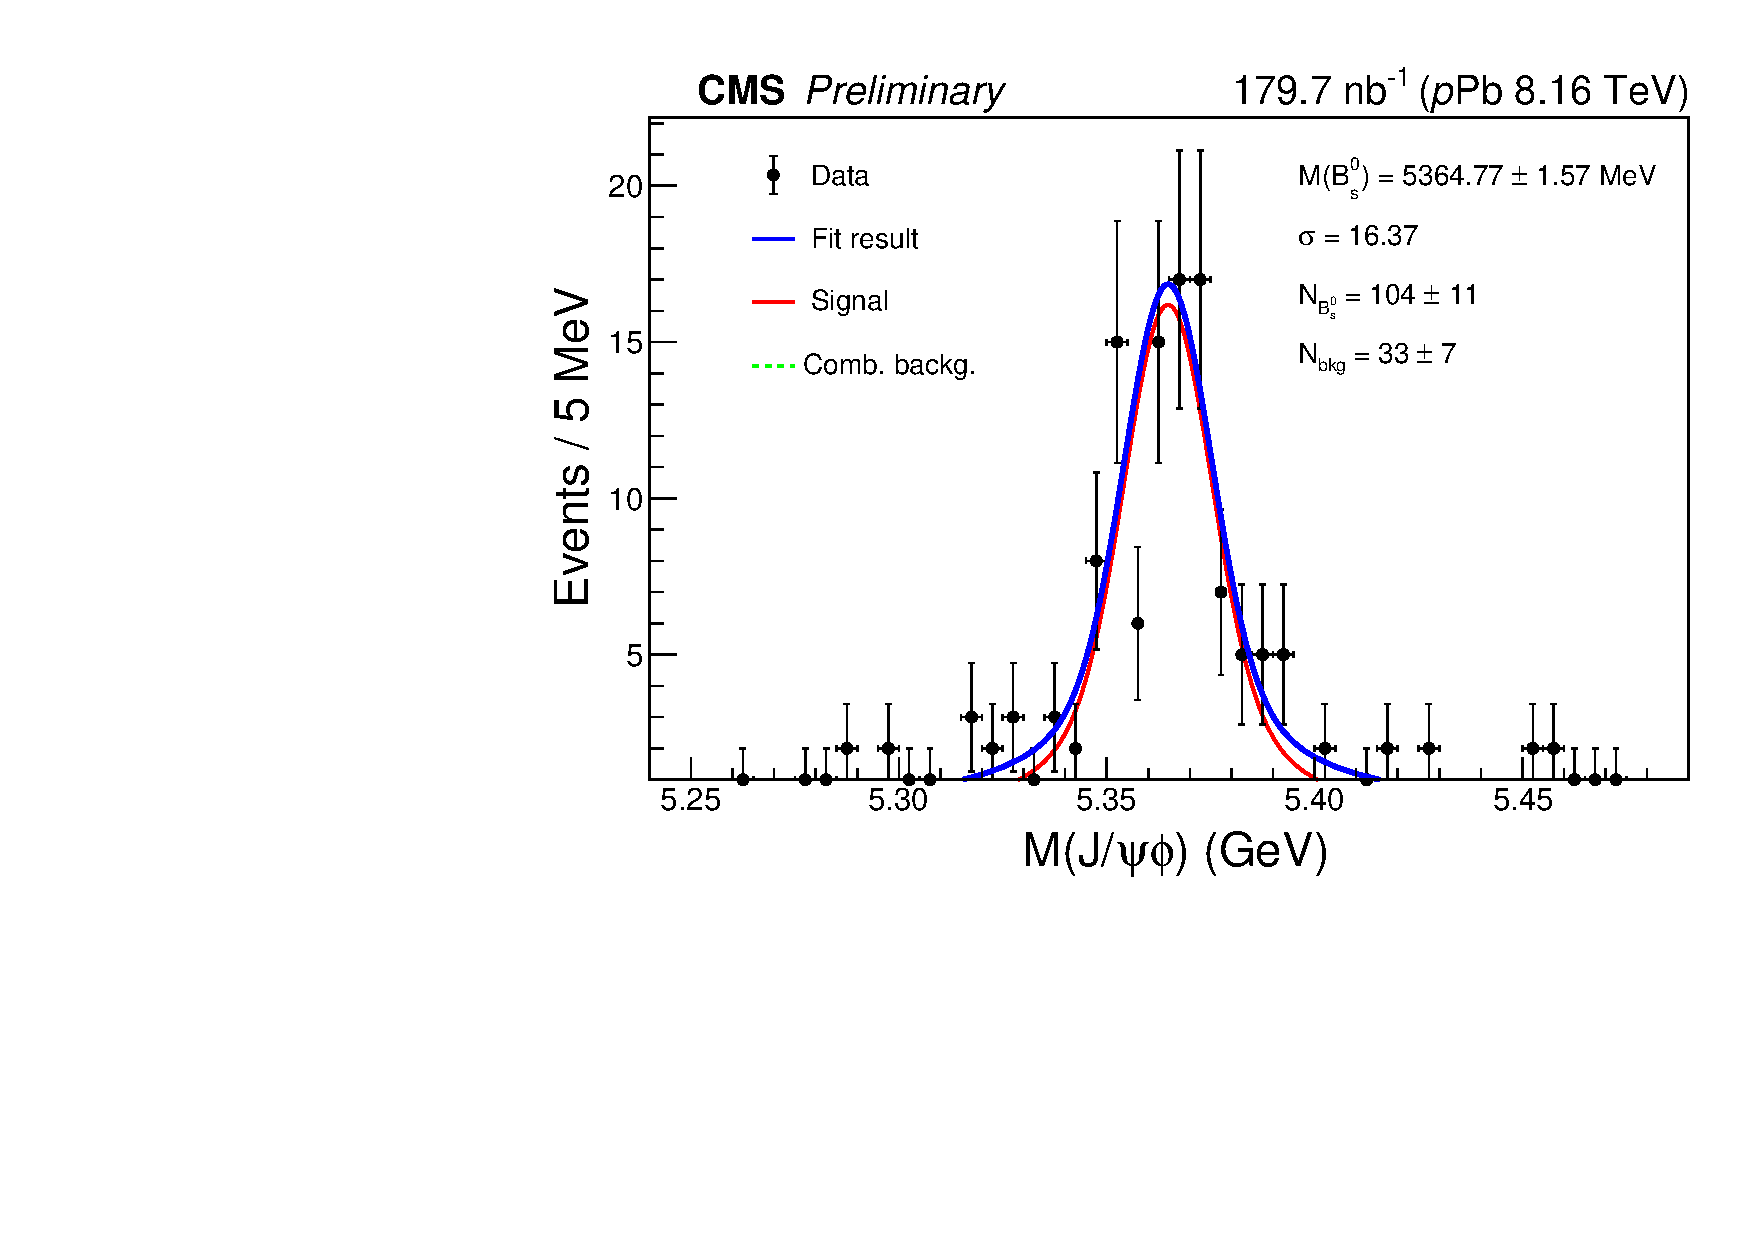
\includegraphics[width=0.49\textwidth]{MainContent/Figs/mass/mass_BsFit_ptbins_sysbkg_20_50.PDF}}%
	\end{subfigure}
	\hfill
	\begin{subfigure}[t]{0.8\textwidth}
		\raisebox{-\height}{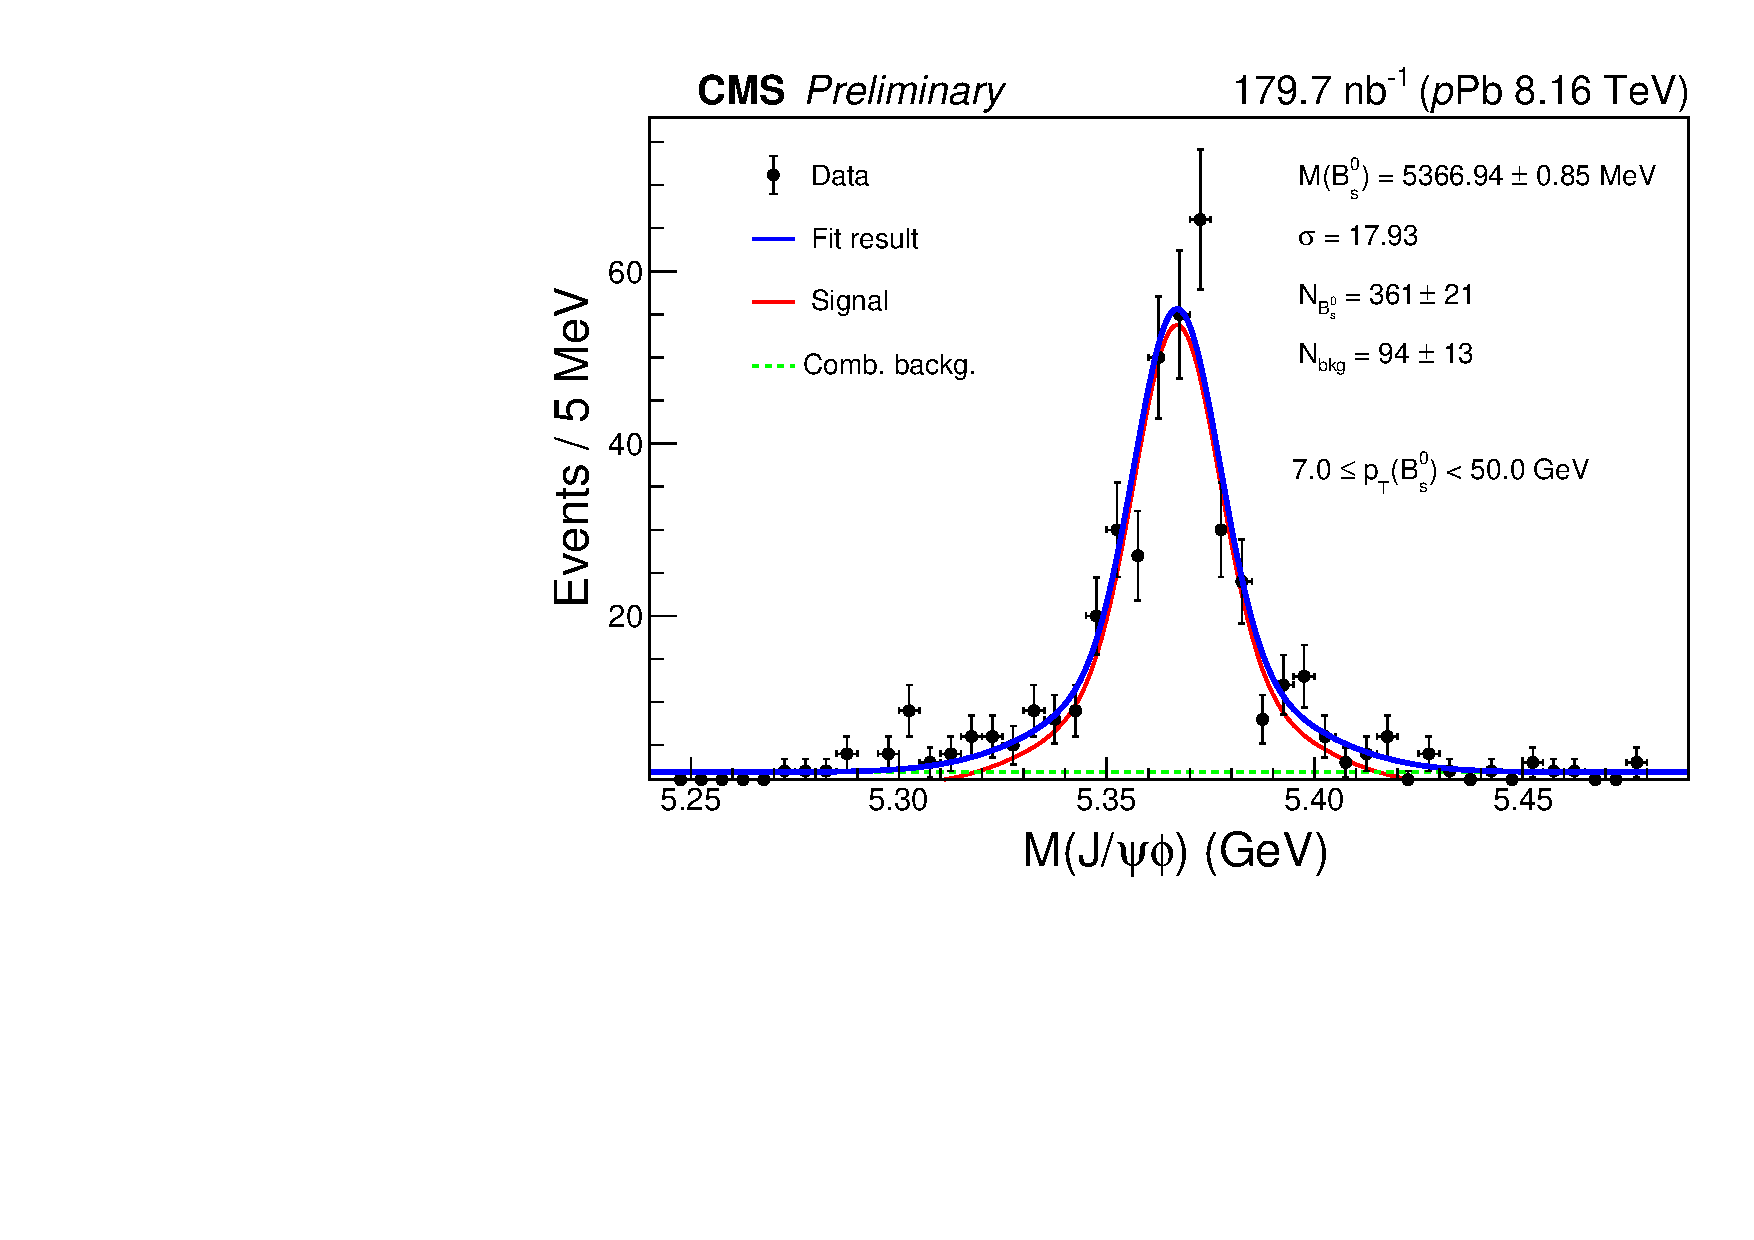
\includegraphics[width=\textwidth]{MainContent/Figs/mass/mass_BsFit_ptbins_sysbkg_7_50.PDF}}
		
	\end{subfigure}
	\caption{Invariant mass spectra for the $B^0_s$ meson using the data from p-Pb collision and a different model for the background data.}
	%%%%%%%%%%%%%%%%%%%%%%%%%%%%%%%%%%%%second row
	
\end{figure}

\begin{figure}
	\centering
	\begin{subfigure}[t]{0.8\textwidth}
		\raisebox{-\height}{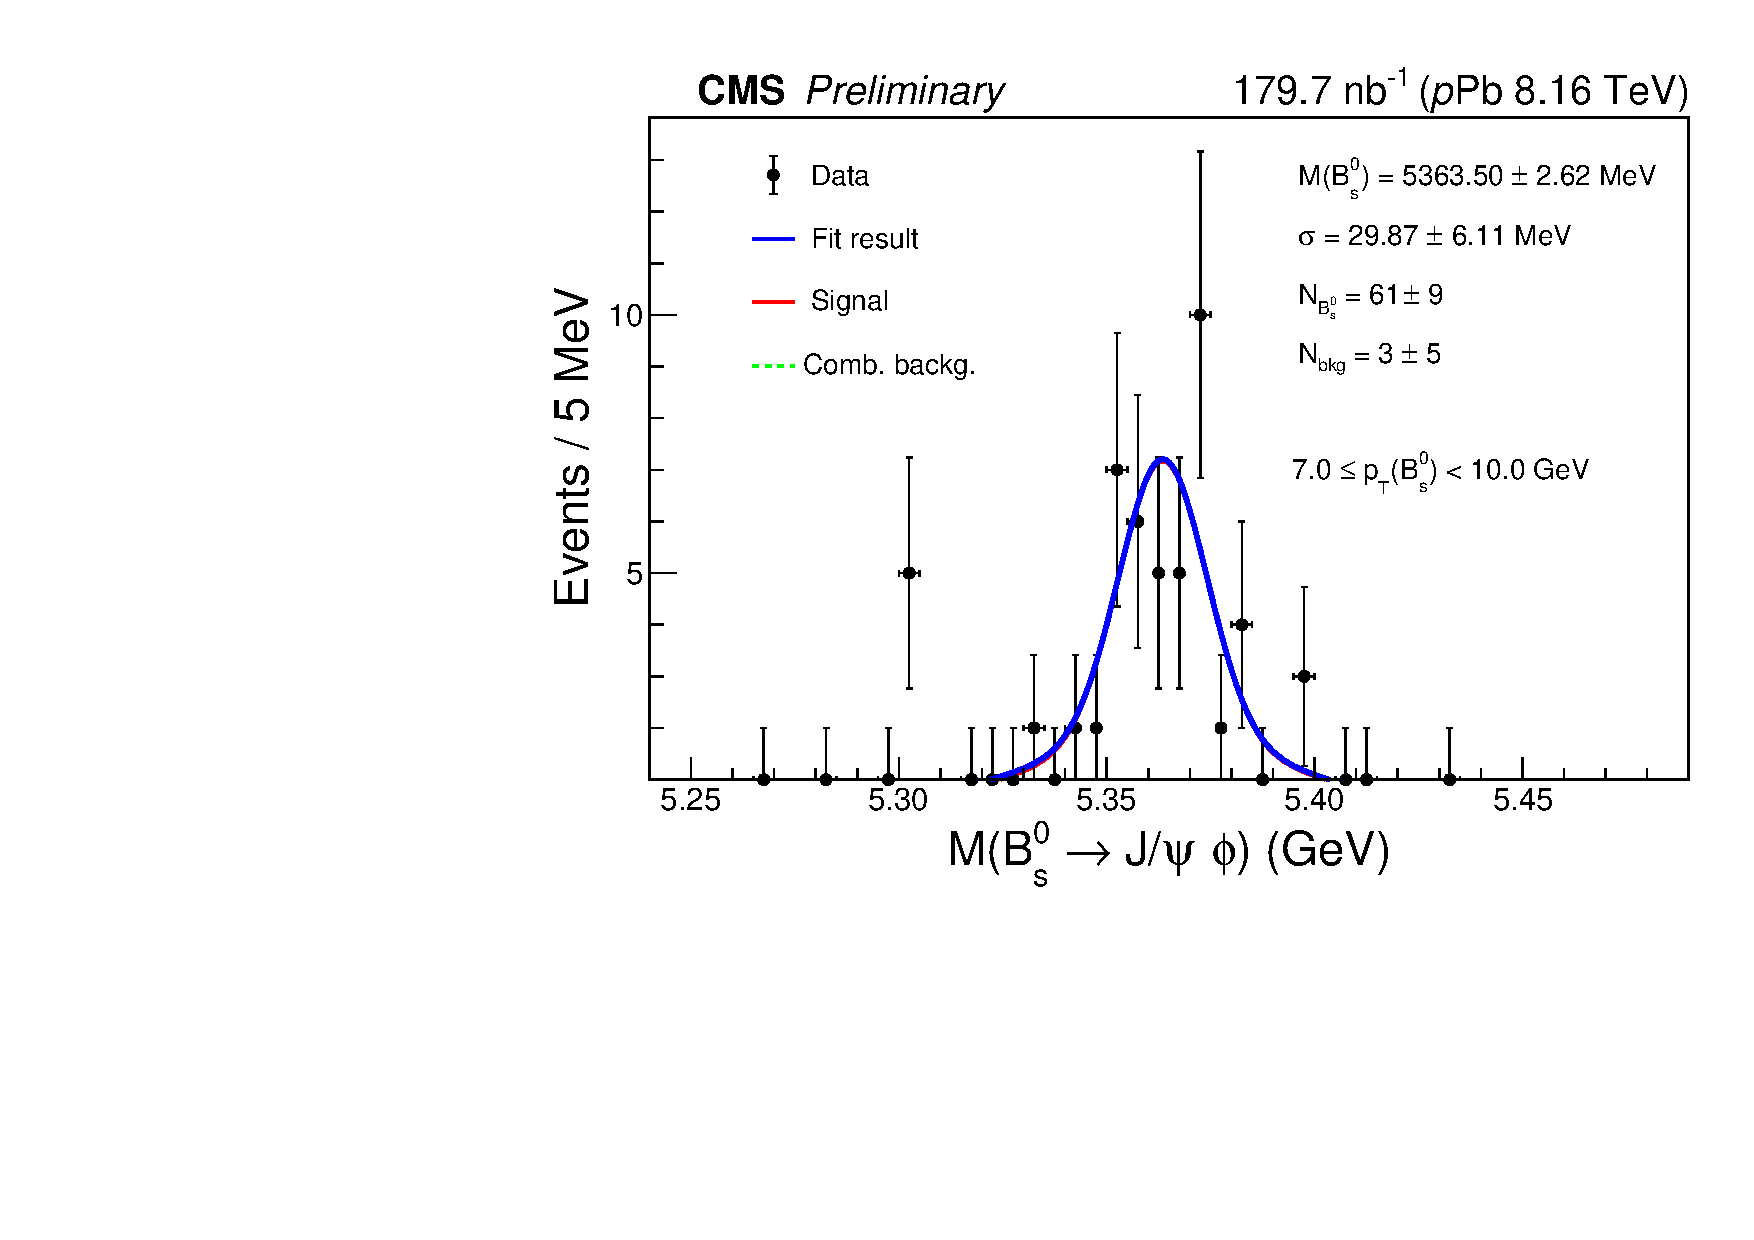
\includegraphics[width=0.49\textwidth]{MainContent/Figs/mass/mass_BsFit_ptbins_syssig_7_10.PDF}}
		\raisebox{-\height}{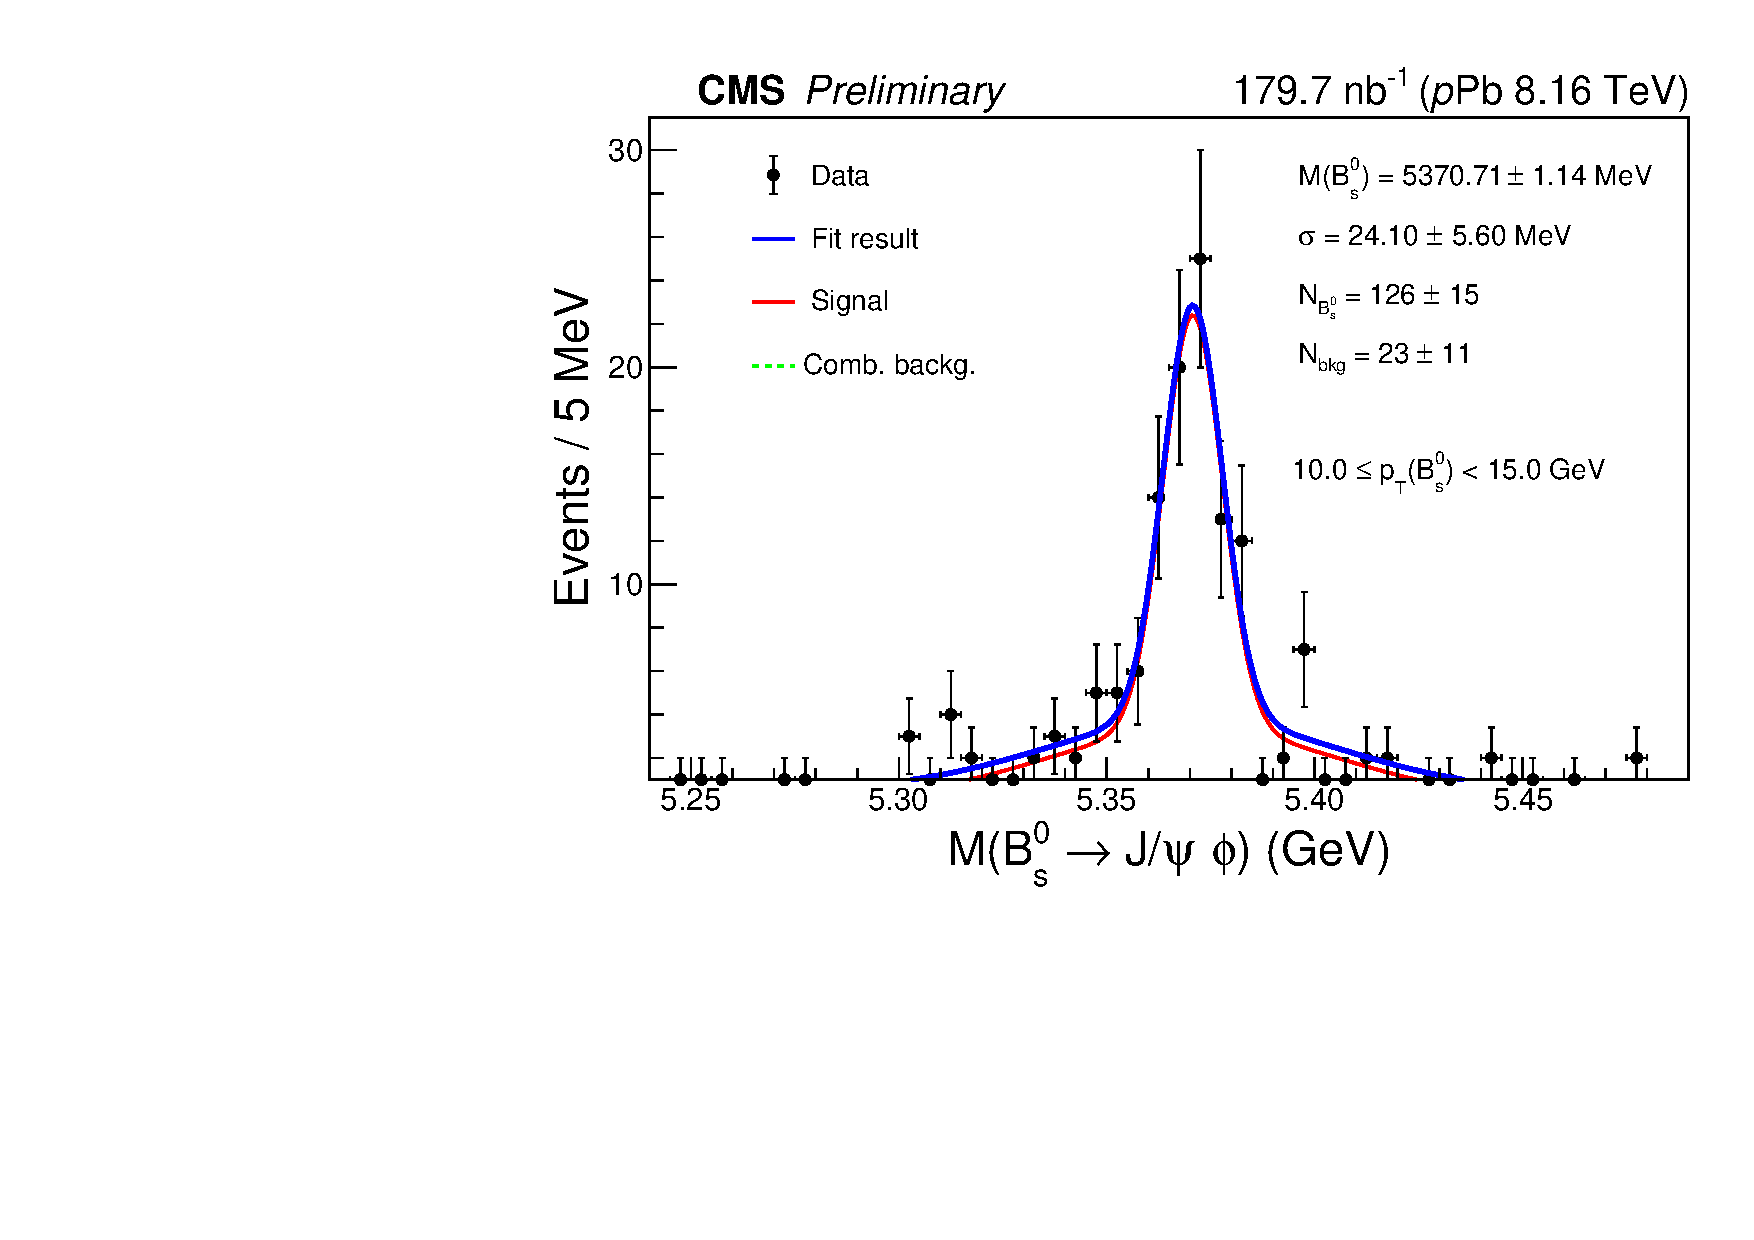
\includegraphics[width=0.49\textwidth]{MainContent/Figs/mass/mass_BsFit_ptbins_syssig_10_15.PDF}}%
		\vspace{.6ex}
		\raisebox{-\height}{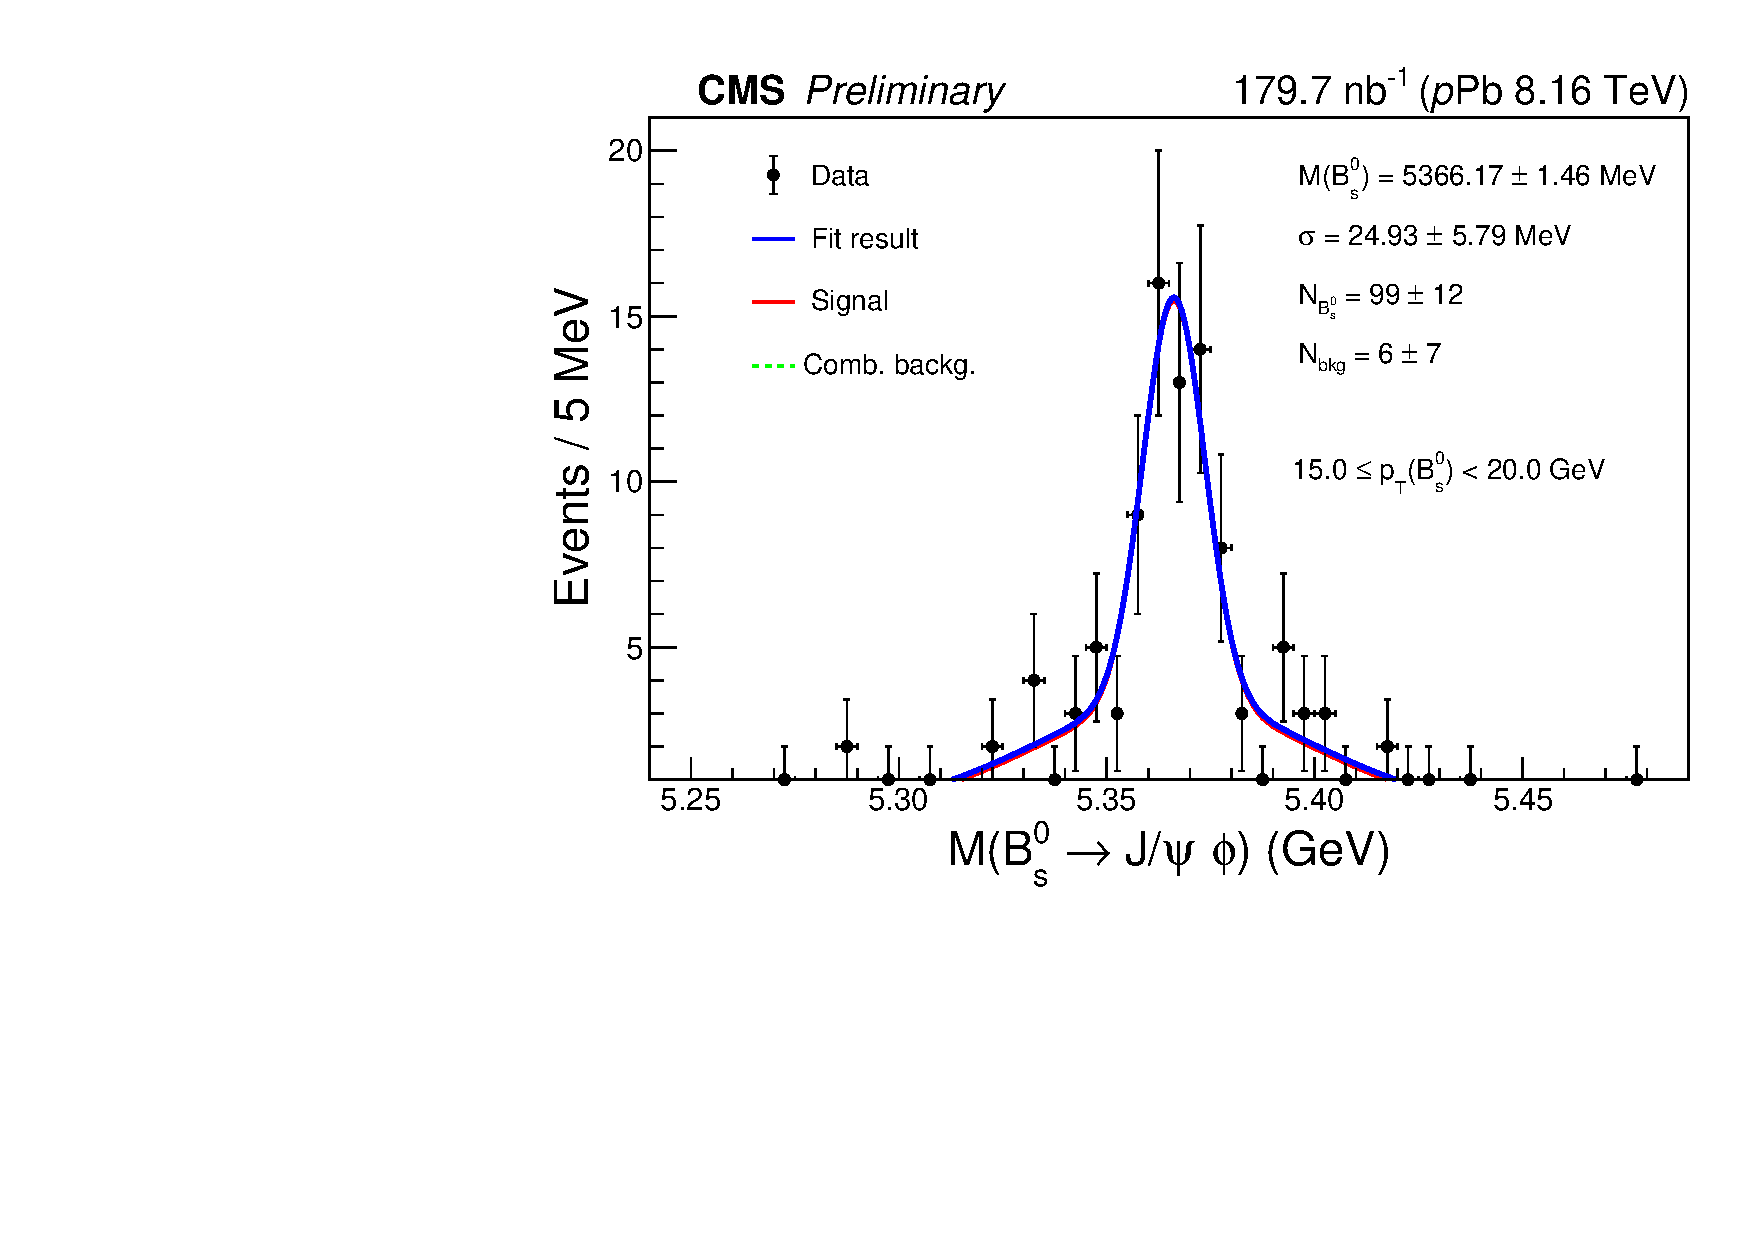
\includegraphics[width=0.49\textwidth]{MainContent/Figs/mass/mass_BsFit_ptbins_syssig_15_20.PDF}}
		\raisebox{-\height}{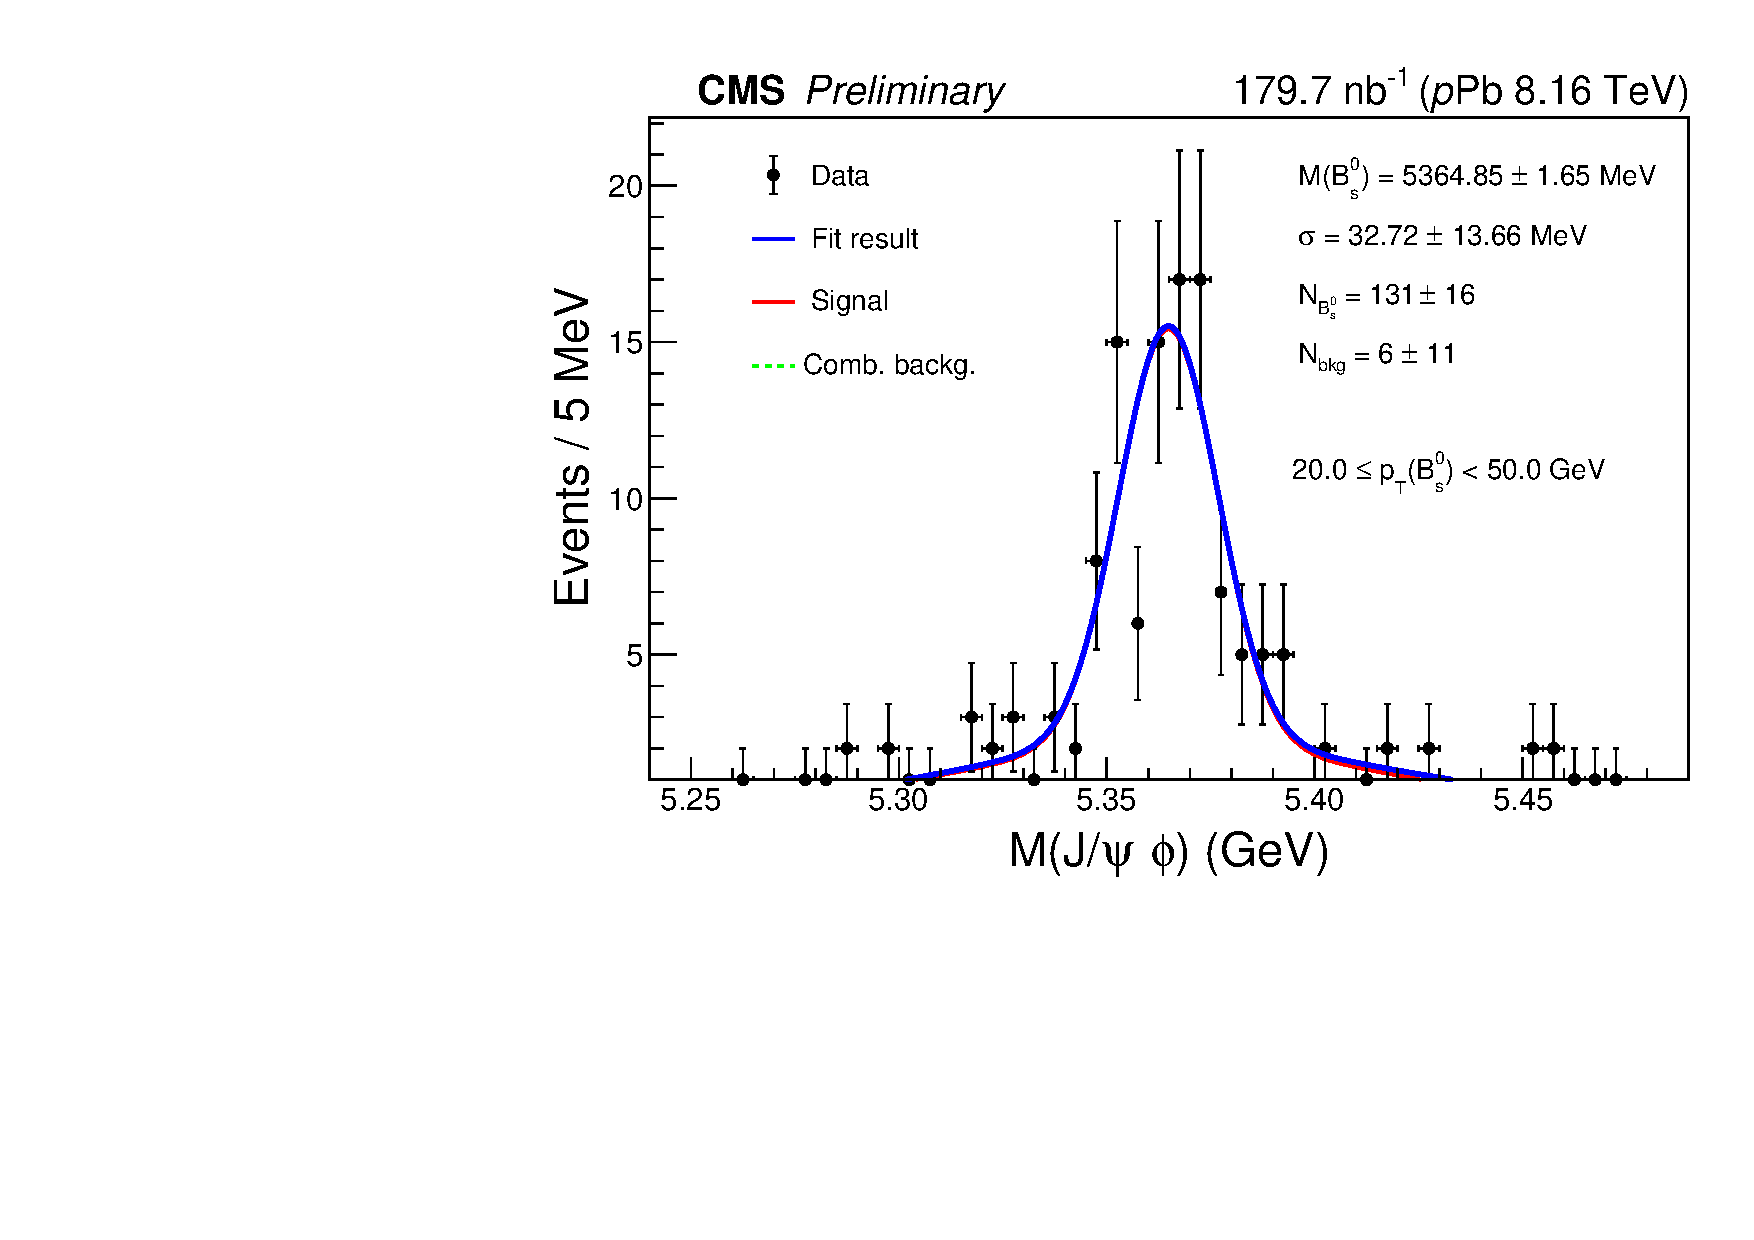
\includegraphics[width=0.49\textwidth]{MainContent/Figs/mass/mass_BsFit_ptbins_syssig_20_50.PDF}}%
	\end{subfigure}
	\hfill
	\begin{subfigure}[t]{0.8\textwidth}
		\raisebox{-\height}{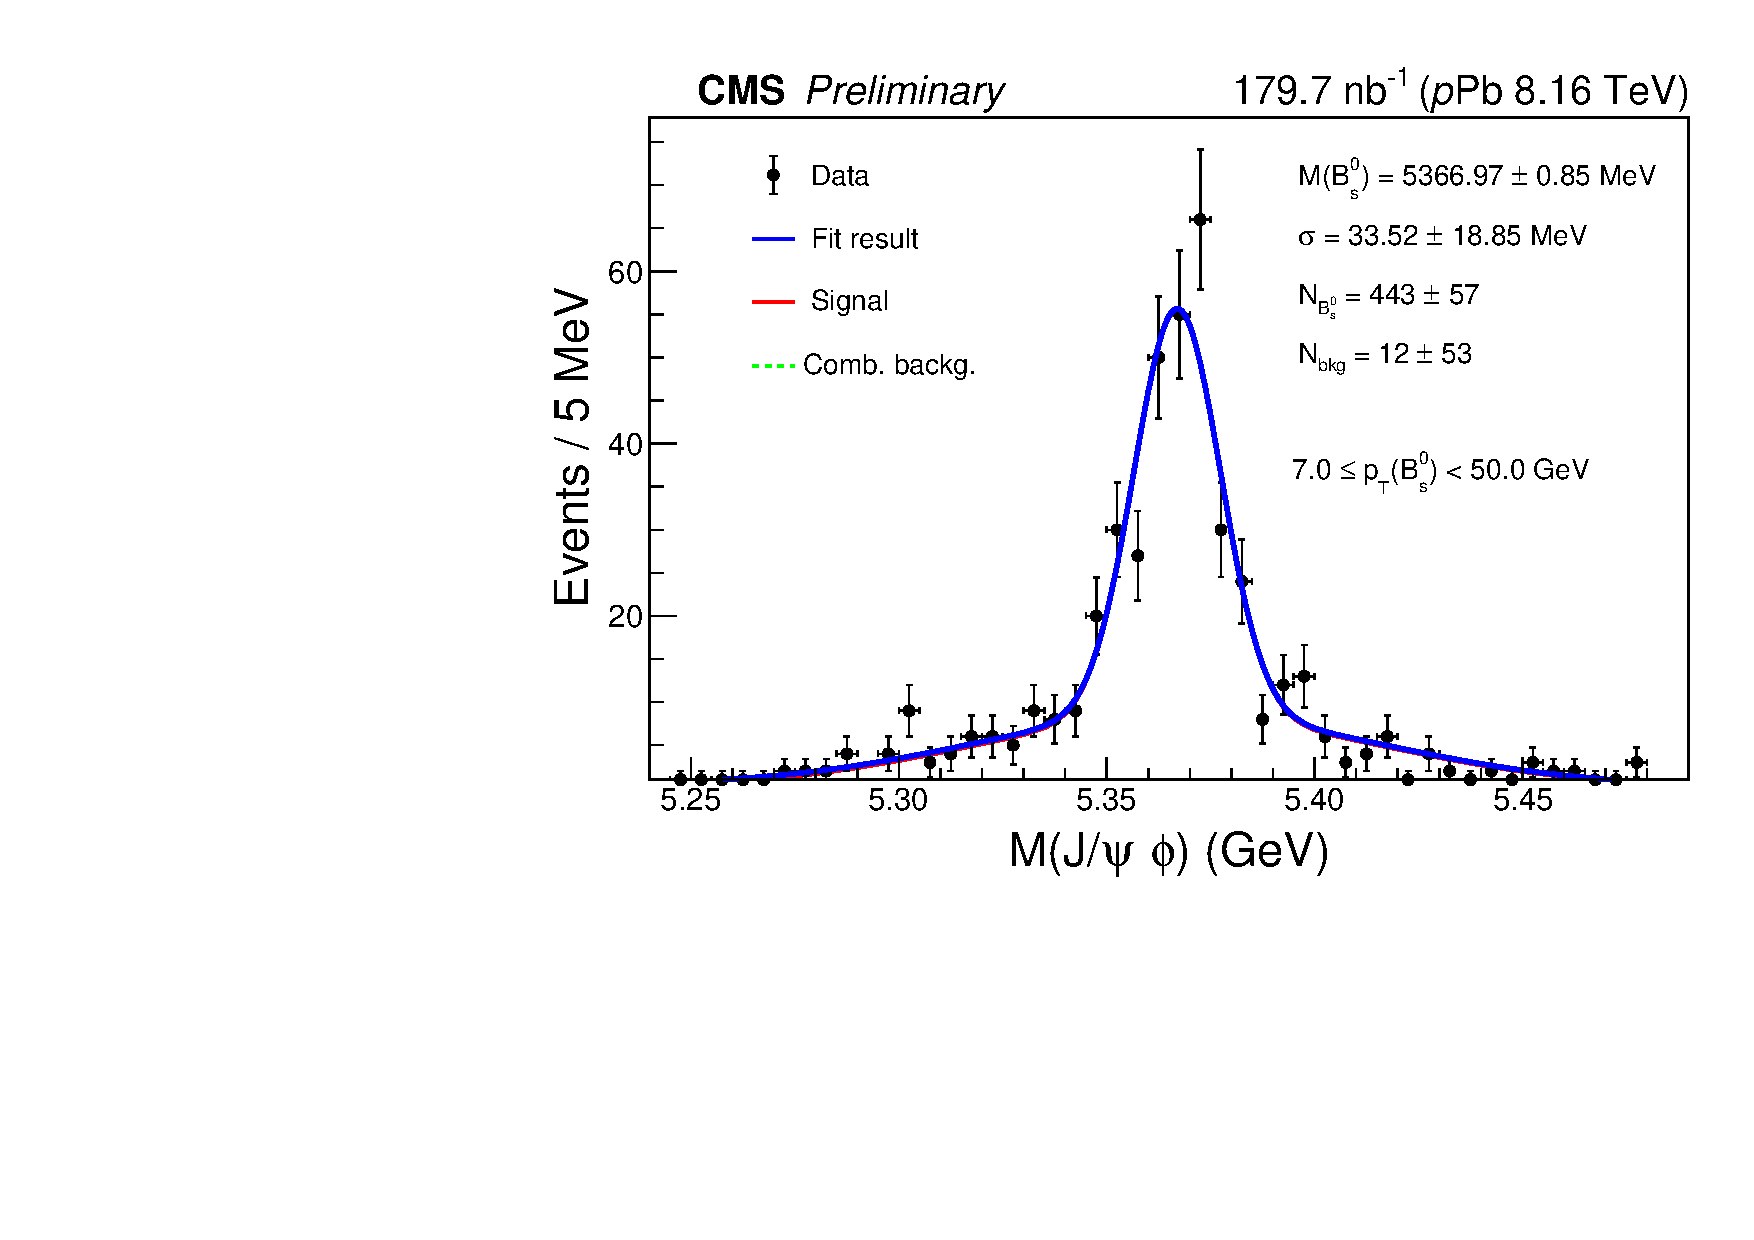
\includegraphics[width=\textwidth]{MainContent/Figs/mass/mass_BsFit_ptbins_syssig_7_50.PDF}}
		
	\end{subfigure}
	\caption{Invariant mass spectra for the $B^0_s$ meson using the data from p-Pb collision and and a different model for the signal data.}
	%%%%%%%%%%%%%%%%%%%%%%%%%%%%%%%%%%%%second row
	
\end{figure}


\subsection{$|y|$ bins}

\section{Total efficiency}

\section{Systematic models}


\section{Differential cross-section}